% !TEX encoding = UTF-8 Unicode
% !TEX TS-program = lualatex
% !BIB TS-program = biber

\documentclass[%
   corpo=12pt, % optional; default:= 10pt
   twoside, % recommended
   tipotesi=scudo,
   mybibliostyle, % only if biblio is typeset with a personal style
  numerazioneromana, % not necessary in a real thesis
   ]{toptesi}
   

\begin{filecontents*}{\jobname.xmpdata}
\Author{Michele Cocca}
\Title{Conversion of FFCS ICE fleet to EV: a data-driven approach}
\Subject{Doctoral dissertations in the SCUDO doctoral school}
\Keywords{PDF\sep
          PDF/A\sep
          ISO 19005\sep
          LaTeX\sep
          PhD Thesis\sep
          Engineering\sep
          SCUDO}
\Publisher{Politecnico di Torino}
\end{filecontents*}
%%%%%%% -----------------------------------------------------------
   
%%%% Use the following package if and only if you want to produce
%%%% an archivable document according to standard PDF/A-1b
%%%% No need to load package imakeidx, because it has already been
%%%% loaded by the specific module toptesi-scudo.
\usepackage[a-1b]{pdfx}
\usepackage[linesnumbered,ruled,norelsize]{algorithm2e}
%%%%%% Read the English documentation of TOPtesi in order to check
%%%%%% the special attention needed to produce ISO compliant
%%%%%% archivable files
%%%%

\ifPDFTeX
    \usepackage[utf8]{inputenc}% 
    \usepackage[T1]{fontenc}
\fi

\errorcontextlines=9% more information on the console in case of errors

%%%% Specify fonts here; chose one among these fonts by leaving just
%%%% one line without initial comment character.
%%%% With LuaLaTeX or XeLaTeX don't change fonts
\ifPDFTeX % using pdflatex
    \usepackage{lmodern} % Default
    %\usepackage{newtxtext,newtxmath}% Times eXtended for text and math
    %\usepackage{fourier}% Utopia, Helvetica and "monospace = ?"

\else % using lualatex (or xelatex)
% Here we use the Libertinus serif, sans serif, monospaced and math fonts;
% they are alla available with a complete up-to-date TeXLive installation.
% Without specifying any OpenType font, the Latin Modern OpenType ones are
% used by default; try commenting the setting for Libertinus Mono, run with
% LuaLaTeX and see what happens; you might prefer to keep the comment sign
% in this line.
    \usepackage{fontspec}
    \defaultfontfeatures{Ligatures=TeX}
    \setmainfont{Libertinus Serif}
    \setsansfont{Libertinus Sans}
    \setmonofont{Libertinus Mono}[Scale=MatchLowercase]
    \usepackage{unicode-math}% add special math stile option here
                             % for example [style=ISO]
% define one math font 
    \setmathfont{Libertinus Math}%
\fi


\usepackage{kantlipsum,mwe} % to produce dummy text and dummy figures



\makeindex[intoc]% collect material to index

%%%%%%%%%%%%%%%%%%%%%%%%%%%%%%%%%%%%%%%%%%%%%%%%%%%%%%%%%%%%%%
% This conditional code is an example of using a different bibliography
% style from the one predefined by the class.
% The usage of the conditional code (also with a different contents) is
% discouraged, because the predefined numbered bibliography style is the
% one generally used in scientific publications.
% Even if discouraged, it is not forbidden.
\ifmybibstyle 
  \usepackage[autostyle]{csquotes} % necessary for biblatex
  \usepackage[backend=biber,
              style=philosophy-classic,
              scauthors=all,
              sorting=nyt,
              natbib]{biblatex} % LaTeX specific bibliography handler
\fi 
\addbibresource{\jobname.bib}% bibliographic data base(s)
% It is recommended to name a single or the primary .bib file with the same
% name as the thesis master file: the macro \jobname contains that name.
% It is possible lo use a comma separated list of bibliographical databases
% but extreme care must be paid to the fact that all .bib files have
% actually different names, and that the citations key are really distinct
% among alla databases, not simply within a single database.
%%%%%%%%%%%%%%%%%%%%%%%%%%%%%%%%%%%%%%%%%%%%%%%%%%%%%%%%%%%%%%
% The following is to be loaded as the end of the preamble if one wants
% to use hyperlinks and/or urls to be typed within the thesis,
% except that after loading hyperref very few commands may be
% issued. One is the \includeonly command with its list of files;
% other packages may be loaded after hyperref, only if their
% documentation says so; some of these critical packages, but they are
% not the only ones, involve Right to Left languages or other
% oriental languages.
%
% Distinguish the hyperref call from the hyperref setup so as
% to avoid option clashes with other packages that may invoke 
% hyperref with different options.

\unless\ifcsname ver@hyperref.sty\endcsname\usepackage{hyperref}\fi
\hypersetup{%
    pdfpagemode={UseOutlines},
    bookmarksopen,
    pdfstartview={FitH},
    colorlinks,
    linkcolor={blue},
    citecolor={blue},
    urlcolor={blue}
  }
%%%%%%%%%%%%%%%%%%%%%%%%%%%%%%%%%%%%%%%%%%%%%%%%%%%%%%%%%%%%%%

%%%% The \includeonly argument should preferably be written with
%%%% one file name per line, so that by commenting or uncommenting
%%%% some lines a selective compilation may be executed.
\includeonly{%
Chapter1/1_introduction,%
Chapter2/2_datacollection,%
Chapter3/3_cs_comparison,%
%Appendix1/appendix1,
%Appendix2/appendix2,%
}
%%%%%%%%%%%%%%%%%%%%%%%%%%%%%%%%%%%%%%%%%%%%%%%%%%%%%%%%%%%%%%
\newcommand{\tool}{\textit{UMAP}\xspace}
\newcommand{\MGM}[1]{#1}
\newcommand{\removelatexerror}{\let\@latex@error\@gobble}

\ifPDFTeX \usepackage{indentfirst}\fi
\raggedbottom

\begin{document}

% The contents of this ThesisTitlePage environment may be written
% in a configuration file named exactly the same as the thesis main
% file, but with extension .cfg. If similar commands with different
% data are written within this environment, such data prevail on
% those read from the configuration file.
\begin{ThesisTitlePage}
% Use the optional command to set a different School logo
% Its is possible to used this command several times; each time
% a new different  Institution logo  may be added. In general
% just the ScuDo logo is sufficient; for dissertations made in
% cooperation with the University of Turin, its logo may be added
% with a second instance of the \PhGschoolLog statement. With
% dissertations supported by the INRiM, this institution logo may
% be added. Such logos (in PDF format) may be obtained from the
% ScuDo web server.
\PhDschoolLogo{scudo}% Fake logo for this example
%\PhDschoolLogo{Logo-ScuDo-blu} % just the ScuDo logo
%\PhDschoolLogo{Logo-ScuDo-blu,Logo-INRIM} %for dissertations made in cooperation with INRIM
%\PhDschoolLogo{Logo-ScuDo-blu,Logo-INFN} %for dissertations made in cooperation with INFN
%\PhDschoolLogo{Logo-ScuDo-blu,Logo-UniTo} %for dissertations made in cooperation with the University of Turin
% Doctorate course name; mandatory
\ProgramName{Electronic and Telecommunication Engineering}
% Cycle ordinal number; optional.
% You can write 29.th, or 29\ap{th}, or 29\textsuperscript{th}, or ...
\CycleNumber{33.th}
% PhD candidate name; mandatory
\author{Michele Cocca}
% Dissertation title; mandatory
\title{Conversion of FFCS ICE fleet to EV}
% Dissertation subtitle: optional.
% It might be useful only if the actual full title is too long.
\subtitle{a data-driven approach}
% The supervisor(s) label; optional; default value "Supervisor:".
% You can change it to plural as in this example, where the colon has
% been eliminated.
%\NSupervisor{Supervisor}{Supervisors}
%
% The SupervisorNumber may contain a value such as 0, 1, or any
% number higher than 1. If 0 is specified, no label is typeset
% over the supervisor(s) list; if 1 is specified then the singular
% form is used: if any value higher than 1 is specified, the plural
% form is used.
\SupervisorNumber{1}
% List of supervisors with academic title, name(s), surname(s),
% and function; mandatory
\SupervisorList{%
    Prof.~Marco Mellia, Supervisor\\
    }
% Name of the examining committee: optional. 
% Default value "Doctoral Examination Committee"
%\Nexaminationcommittee{Doctoral examination committee}
% List of the  examining committee members: mandatory if the above label
% is not empty.
\ExaminerList{%
Prof.~A.B., Referee, University of \dots\\
Prof.~C.D., Referee, University of \dots\\
Prof.~E.F., University of \dots\\
Prof.~G.H., University of \dots\\
Prof.~I.J., University of \dots}
% Name of the institution where the examination takes place; optional.
% Default value: "Politecnico di Torino"
%\Nlocation{Politecnico di Torino}
% Examination date: mandatory, although the way to write it is free.
\ExaminationDate{\today}
% Disclaimer with signature; optional. Default text as
% in the following lines. 
\Disclaimer{%
\noindent I hereby declare that, the contents and organisation of this dissertation constitute my own original work and does not compromise in any way the rights of third parties, including those relating to the security of personal data.	
}
%\Signature{%
%\begin{flushright}
%\parbox{0.5\textwidth}{\centering
%\dotfill\\
%Mario Rossi\\
%Turin, February 29, 2123
%}
%\end{flushright}}
\end{ThesisTitlePage}
%%%%%%%%%%%%%%%% Everything else necessary in the thesis title
%%%%%%%%%%%%%%%% page and in the copyright page is supplied by
%%%%%%%%%%%%%%%% the default values.
%%%%%%%%%%%%%%%% If you enter an explicit disclaimer, you can
%%%%%%%%%%%%%%%% typeset other material before the disclaimer
%%%%%%%%%%%%%%%% formula; use the necessary spacing on order
%%%%%%%%%%%%%%%% to separate the formula from other text. 
%%%%%%%%%%%%%%%% 
%%%%%%%%%%%%%%%% For example you might want to write the formal
%%%%%%%%%%%%%%%% statement for a particular licence, provided the 
%%%%%%%%%%%%%%%% licence allows Open access; not necessarily all uses
%%%%%%%%%%%%%%%% of the thesis should be allowed, but the minimum
%%%%%%%%%%%%%%%% is the reading access.

%%%%%%%%%%%%%%%% The next two lines are metadata for a normal PDF file.
%%%%%%%%%%%%%%%% For ISO archivable PDF/A-1b metadata, they must
%%%%%%%%%%%%%%%% be entered only in the form used in the file
%%%%%%%%%%%%%%%% named in the filecontents* environment as shown
%%%%%%%%%%%%%%%% at the beginning of this file.

%\subject{How to typeset a doctoral thesis suitable for defence in almost any country and university.}
%\keywords{{pdfLaTeX} {LuaLaTeX} {XeLaTeX} {PhD doctoral programs} {PhD dissertation} {Politecnico di Torino}} 

\summary%\sommario

This is where you write your abstract \dots\ (Maximum 4000 characters, i.e. maximum two pages in normal sized font, typeset with the thesis layout).

The abstract environment is also available, but  \texttt{\string\summary} is preferred because it generates an un-numbered chapter. The abstract environment is more suitable for articles and two column typesetting without a separate title page.

\emptypage %  it works even without the classica option
\acknowledgements% or \ringraziamenti

And I would like to acknowledge \dots

Acknowledgements are mandatory only when people outside the academic institution supported the development of the research that was performed in order to reach the conclusion of the doctorate program.

\begin{dedication}

\textit{I would like to dedicate this thesis to my loving parents} 

{\normalsize 
The dedication very seldom is a proper thing to do; in some countries it is very common, while in other countries it is done for imitation of other people habits. 

The sentence used above clearly is an example of something very common, but it is  useless. Of course we all love our beloved parents, but it is not necessary to ``engrave it in stone''.
\par}
\end{dedication}
%\end{dedica}

%%%%%%%%% If you want these two lists, uncomment the following line
%\tablespagetrue\figurespagetrue % 

%%%%%%%%% Table of contents and optionally the tables and figures lists
\allcontents

\mainmatter %all the above is front matter; here begins the main matter

% !TEX root = ../toptesi-scudo-example.tex
% !TEX encoding = UTF-8 Unicode
%***********************************************************************
%*********************************** First Chapter 
%***********************************************************************

\chapter{Introduction}  %Title of the First Chapter
\label{chap:1_introduction}
    \graphicspath{{Chapter1/}}


descrivo la storia i benefit e la storia del carsharing



% !TEX root = ../toptesi-scudo-example.tex
% !TEX encoding = UTF-8 Unicode
%***********************************************************************
%***********************************Second Chapter
%***********************************************************************

\chapter{Data acquisition}
\label{chap:2_dataset}
	\graphicspath{{Chapter2/}}

Car sharing is nowadays a popular means of transport in smart cities. In particular, the free-floating paradigm lets the customers look for available cars, book one, and then start and stop the rental at their will, within a specific area. This is done thanks to a smartphone app, which contacts a web-based backend to exchange information. In this paper we present \tool, a platform to harvest the data freely made available on the web by these backends and to extract driving habits in cities.

We design \tool with two specific purposes. Firsty \tool fetches data from car sharing platforms in real time. Secondly, it processes the data to extract advanced information about driving patterns and user's habits. To extract information, \tool augments the data available from the car sharing platforms with mapping and direction information fetched from other web platforms. This information is stored in a data lake where historical series are built, and later analyzed using analytics modules easy to design and customize. 

We prove the flexibility of \tool by presenting a case of study for the city of Turin. We collect car sharing usage data for over 50 days to  characterize both the temporal and spatial properties of rentals, and to characterize customers' habits in using the service, which we contrast with public transportation  alternatives. Results provide insights about the driving style and needs, which are useful for smart city planners, and prove the feasibility of our approach.


\section{Introduction}
\label{sec:intro}

Mobility is one of the challenges to solve in our society and in cities, where eco-sustainability is becoming more and more important. 
Regulators and policy makers are positively looking into ``smart'' approaches to improve the current status of their urban network.  The ability to collect data, is the first step to take informed decisions. Unfortunately, getting information about mobility patterns and human driving habits is not easy because of both technical challenges and privacy issues.

To this extent, in this paper we investigate the possibility of harvesting data openly exposed on the Web to obtain information about mobility habits in cities, and make it available to the players by using a smart-platform. We focus on car sharing platforms and mapping and direction services.
%
%For many years the usage of a private car for transportation was the most important solution. Nowadays this trend seems to decrease, especially among young adults for who owning a private car look to be less important. This change to alternative mobility services favorites the growth of car sharing systems.
%
%The first known solution of such a system is the Selbstfahrergenossenschaft car  sharing program born in 1948 in Zurich without a former development of it. Only in the early 1970s saw a first system based on car sharing. However, only recently, with the growth of the sharing economy, the car sharing system accelerated its growth, making nowadays the car sharing widely used in different parts of the world. As a matter of fact, the importance of car sharing systems is demonstrated by the expansion in term of mermership number. According to~\cite{a,b} this growth exceeds 10\% per year either in North America and Germany.

%Among the key advantages of such a system, has been proved that it allows traffic and pollution reduction~\cite{}.

Car sharing refers to a model of car rental where customers rent a car for a short period of time, usually for a few hours or less. One of its most interesting systems is the so called \textit{Free-Floating Car Sharing (FFCS)} system. The peculiarity of this system is that customers can pick and drop the car wherever in a geo-fence area.
The most famous company is car2go which is present in 25 cities and 8 different countries, both in Europe and North America.

%, where customers rent a car via the web or a smartphone app
% In the station-based approach, users have to pick-up the car and release it in specific positions e.g., parkings spot reserved for this car. A first example of this system is the famous American \textit{Zipcar} service, which allows users to pick up the car in specific parking spots and then return the car in the same starting point. An alternative is the one-way solution, like  \textit{Autolib'} in Paris, an electrical car sharing system where users can rent a car in one station and return to a different one. The peer-to-peer solution is based on the idea that most private car are most of the time unused(90\% of the time according to some estimation~\cite{c,yltechrep}). In this model, cars are made available by private users. The company which manage this kind of service only takes care of providing the insurance and finding customers to rent the car. This system is quite new to the market and it is exploited by a few companies (the most important one is RelayRides, in the US).
%
To rent a car in a modern FFCS system, users check on their smartphone, or on the FFCS website, which cars are available in the neighborhood. Then, with a simple tap they can book a car, and start/end the rental. The FFCS app contacts a web-based backend server to fetch data about available cars, perform a booking, and accounting operations. Typically for this purpose web API are used, some of which are publicly documented~\cite{car2goAPI}. The same website and app offer information about the status of the car rental systems, and the same web API can be used to collect for free this information. In the past, this approach has been successfully used to obtain data for specific mobility studies -- see Sec.~\ref{sec:related} for more details.
In this work, we extend this idea and focus our attention on the acquisition and harvesting of this data by means of big data techniques to understand driving habits in a city. We take the city of Turin as a use case.

We design \tool, a platform to collect, process, augment, and store data in a data lake, where analytics let the analyst extract higher level information.
We build two crawlers to collect data from the \textit{car2go}  and \textit{Enjoy} platforms\footnote{\url{www.car2go.com}, \url{enjoy.eni.com}}, both present in Turin. Every minute, the crawler checks which cars are currently available. Every time a given car ``disappears'', it records the booking start time. The same booking ends when the crawler sees the car available back on the system. Some booking are actual ``rental'' in case the car moved from the prior parking position to another. Ingenuity must be used, e.g., to filter GPS fix issues (which may erroneously let a car ``move''), or to handle possible data collection issues (e.g., the website going down, or some cars undergoing in maintenance), or platform design (e.g., synchronous or asynchronous updates).

We let the crawler run to collect data for 52 days, from December 10th 2016 to January 31st 2017. We observed more than 104,000 \textit{bookings} and 86,000 \textit{rentals} for car2go, and 93,000 \textit{bookings} and 81,000 \textit{rentals} for Enjoy. 
%Then, we characterize how user booked or rented the car during such a period, discovering that during the business day FFCS systems are used much more with respect to the weekend. To have a better understating on what is the trend during these two parts of the week, we then characterize the rentals dividing the week in two and studying the trend per hour. We discovered that while during weekdays the system is quite unused during the night, during the weekend we observe twice as much rents with respect to during the week days, but with a reduction during the day especially in the morning. Then, we characterize for how long time users rent cars and how far they go. Interestingly, we first discovered that despite the different pattern between week days and weekend days, the time and the distance users use to use a car does not change. Secondly, we observed that users using car2go use the car also for longer trip due to the possibility to drop the car in the Airport parking lot. By analyzing the duration time in case of bookings without a rental instead, we observed that the higher probability is less then 5 minutes and then at 20 minutes for car2go and around 15 minutes for Enjoy. While the first can be explained by a system fault, the second cases depends on the maximum \textit{reservation time} i.e., the maximum time an user can reserve a car without paying any fee. 
With these datasets, we characterize the FFCS service utilization, in terms of bookings and rentals, with the aim to observe how people use these services, where they typically go, when, for how long the rental last, etc. Some observations are quite intuitive, e.g., people appear to be willing to use more the FFCS during weekdays and during peak-time. Counterintuitively, the rental duration and the driving distance show marginal changes over the day and weeks.

%When comparing the two platforms, we discover that car2go users \DG{sometimes} drive the car for longer trips than the Enjoy users. This is partially due to the possibility to reach the Airport with car2go but not for Enjoy. We also observe that the usage increases during weekend evenings. Both effects suggest a lack of public transport which may be considered by the municipality for improvements.

% By analyzing the duration time of all the bookings that do not describe a rental, we observe that the highest percentage of them have a duration equal or lower than 5 minutes,  other common values are 20 minutes for car2go and around 15 minutes for Enjoy. While the shortest interval can be explained by a system fault or a booking cancellation, the other durations time can be linked with the maximum \textit{reservation time} i.e., the maximum time an user can reserve a car without paying any fee. 

%\DG{MESSAGGIO HEATMAP TBD}

We complement the analysis by comparing the booking duration with the driving duration as suggested by Google Directions application, which we collect in real time for each rental. This allows us to find that 8.5\% of bookings last less than the Google driving time. 
This may be due to Google Directions overestimating the driving duration or, recalling that bookings  include the reservation time and the time to look for a parking spot, this may suggest that the time-based tariffs adopted by FFCS systems may encourage fast driving styles in the hope to reduce the rental cost.
We next compare the duration of the booking with the equivalent trip duration by public transport as returned again by Google Directions. We discover that rentals are 36\% shorter on average than public transport time, but  rentals start to be preferred when public transport time is higher than 10 minutes.

We presented our results to the Turin Transportation Authority, who found them to be extremely useful to understand people driving habits. We believe that \tool represents an important support tool for the investigation of car sharing users' habits. The scalable design of \tool allows the policy maker to collect data from many FFCS providers  and integrate it with other sources. This eases the analysis when taking in consideration trends and providers comparison. \tool allows the Transportation Authority to take informed decisions when planning public transport systems. This characteristic strengthens the potentiality of \tool for economical and sociological prediction and analysis. Our data-driven approach, combined with other more traditional tools like surveys, represents an interesting observation point for understanding potential services improvements, both for car sharing and public transport systems. We make available the source code of \tool for research purposes.\footnote{\url{github.com/MobilityPolito/}}

The reminder of this paper is structured as follows: Sec.~\ref{sec:related} discusses the related work. 
Sec.~\ref{sec:methodology} describes in details \tool data acquisition and analysis capabilities. Sec.~\ref{sec:results} presents our results: First, we characterize car2go and Enjoy car usage over time; second, how customers drive the cars and how they move in the city; finally, we show what are the users' driving habits and the correlation between booking time and the public transport time. Sec.~\ref{sec:conclu} concludes the paper.




\section{Data Acquisition}
\label{sec:2_3_data_acquisition}
\begin{figure}[h!]
\centering
%left top right top
 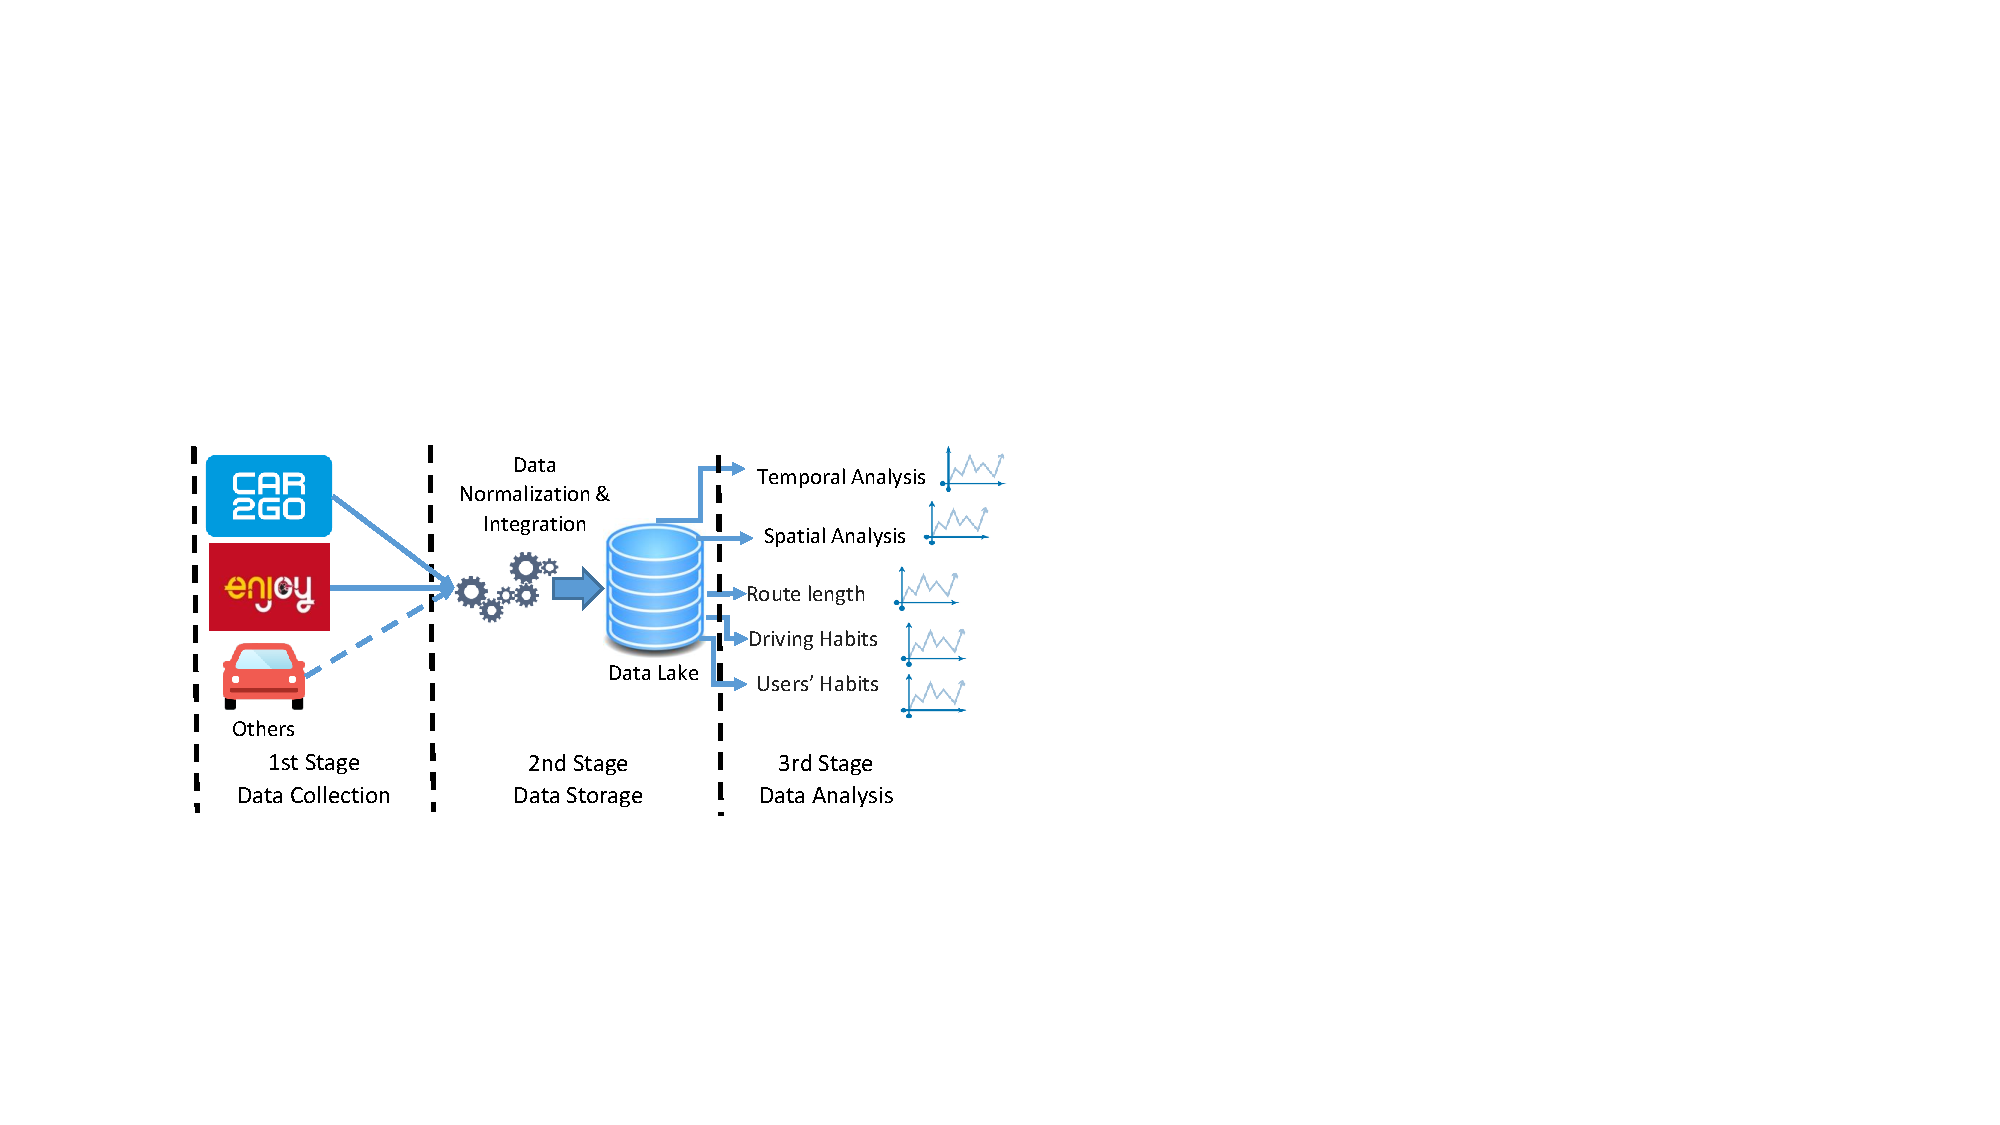
\includegraphics[trim=3cm 4.5cm 17cm 7.2cm,clip, width=0.95\columnwidth]{figures/framework_schema.pdf}
 \caption{\tool overview\label{fig:2_3_c2_framework}}
\end{figure}


In this section, I provide a description of \tool structure. Figure~\ref{fig:2_3_c2_framework} depicts the architecture of \tool, composed by a first module for the data acquisition, by a second module for data normalization and integration, and then a third  module for the data analysis.

The first module consists in the data acquisition from the car sharing platforms of interest. These typically expose information about cars' location when available for rental through a web-service approach. 

For this module I design two crawlers, one for the car2go and one for the Enjoy car sharing platforms. They retrieve, at each time instant, which cars are available in a given city.

While car2go offers public APIs~\cite{car2goAPI}, Enjoy does not provide to users such a service. For this reason I reverse engineer the Enjoy web portal. By leveraging the Chrome Developer Tools, I investigate the information exchanged with the Enjoy web portal while asking the list of available cars. Through this analysis, the software obtains both the URL used to request the list of available cars, and how fetch the data for a specific city.
Both system return the currently available cars using a JSON file.

Each time the system downloads a JSON, a \textit{snapshot} describing which cars are parked and ready for rental. Basically, the \textit{snapshot} is a list containing all cars and their attributes.

In a nutshell, a car is described by the car sharing web-service as an object annotated by several information, like plate, vehicle identification number (VIN), location, fuel level, model, etc. 
All the data represented in this object is useful for the customers e.g., to choose which car to rent.
This object is only present if the car is available, i.e., it is parked and free for a rental. Its state changes over time. In particular, a car disappears when a customer reserves and rents it, and then it reappears when the customer ends the rental (likely in a different location).


At each time $t$, the software gets the JSON snapshot $S$ listing the available cars. 
%We take a snapshot \textit{$S$} every minute to balance aggressiveness of the crawler, and time resolution. 
%At each time t, we obtain from each platform the JSON snapshot S detailing the available cars. 
The sampling period has been set to one minute, to balance aggressiveness of the crawler and a reasonable time resolution.
$S$ describes each available car with several fields, some of them being in common between the considered companies, but in general with different format.
For this study, I collect each car unique identifier and current geo-location indication.
These are obtained from the \textit{VIN} or \textit{plate} field, and the \textit{coordinates} field which describes the \textit{longitude} and the \textit{latitude} of the in-car GPS used to localize it when  parked.\footnote{The GPS coordinates are only available if a car is parked and available. There is no risk for users' privacy during rentals. In addition no user's identifier is exposed. Therefore data is totally anonymized as there is no means to know who booked a car.}
In addition to these fields, the car sharing JSON description may provide other information, e.g., the \textit{street address} corresponding to the coordinates, the \textit{fuel} level, the \textit{car interior status} the \textit{engine type}, etc. Since each platform uses its own data and format, I design a data integration step to have common names for fields containing the same information, if present.

\section{Data Normalization and Integration}
\label{sec:2_4_data_normalization}
In this second module I illustrates hoe \tool processes and consolidate each snapshot to obtain \emph{parking} and \emph{bookings} periods for each car. A \emph{parking} is time where the car is available for a user ride. On the other hand a \emph{bookings} is time elapsing two parking where the car is not tracked by the system. The intuition is to track the availability of each car on the car sharing platform, and rebuild the historic parking and booking periods over time: when a customer books a car, the latter ``disappears'' from the system. The framework records this event, with the initial time and position of a new booking. When the customer ends the booking, the car ``reappears'' in the system. The software records this event, with the final time and position of the booking. For the same car, a new parking period starts.

Harvested data is unstructured, and may grow large. Thus I leverage on \textit{MongoDB}, a NoSQL document-based database. A MongoDB database includes a set collections, i.e., groups of documents. Each document is a set of key-value pairs, organized in a JSON structure. The schema-less structure of MongoDB fits well in this work, because it can handle in the same collection documents defined with different key-value pairs. I decide to rely on such a system as I can easily manage the different field structures of providers, car2go and Enjoy in this use case. In addition, MongoDB offers a great integration with Python through the \textit{pymongo} module.

Four different collections compose the MongoDB data lake:  \textit{ActiveBookings}, \textit{ActiveParkings}, \textit{PermanentBookings}, and \textit{PermanentParkings}. 
\textit{ActiveBookings} and \textit{ActiveParkings} are collections used to store information about the current status of cars (currently booked or parked respectively). These are temporary structures that make it easier to query each car last observed status, and update it. These are also instrumentals for a real-time analysis of the system, e.g., to count how many cars are currently booked or available.
\textit{PermanentBookings} and \textit{PermanentParkings} collections store the history of past state of cars, for past bookings and parkings, respectively.

For the documents in the bookings collections I augment information by inserting also the expected route driving time, and the public transportation duration on the same origin-destination pair. These two piece of information are obtained through the Google Directions API using the initial and the final coordinates as indication of the path.

The most important fields in the \textit{ActiveBookings}, and the \textit{PermanentBookings} collections are:
\begin{itemize}
\setlength\itemsep{0.1em}
\item \textit{CarID}: the unique identifier of the car;
\item \textit{InitTime}: the initial time of the booking;
\item \textit{FinalTime}:  the final time of the booking;
\item \textit{InitCoords}:  the GPS coordinates of the booking star location, i.e., where the users picked up the car;
\item \textit{FinalCoords}:  the GPS coordinates of the parking location where the car was dropped at the end of the booking;
\item \textit{DrivingTime}: The duration of the trip, expressed in seconds, as estimated by Google Directions API, following the best path;
\item \textit{PublicTransportTime}: The duration is expressed as arrival time of the best public transport trip, as estimated by Google Directions API, minus the \textit{InitTime};
\end{itemize}

Instead, the \textit{ActiveParkings} and the \textit{PermanentParkings} collections are characterized by the following fields:
\begin{itemize}
\setlength\itemsep{0.1em}
\item \textit{CarID}: the unique identifier of the car
\item \textit{InitTime}: the initial time of the parking
\item \textit{FinalTime}:  the final time of the parking
\item \textit{Coordinates}: the GPS coordinates of the parking spot 
\end{itemize}

\begin{figure}[t!]
 \removelatexerror
 \scriptsize
  \begin{algorithm}[H]
   	\caption{Data acquisition at time $t$}
	\SetKwInOut{Input}{Input}\SetKwInOut{Output}{Output}
	\Input{$t$ - Current timestamp}
	\Input{$S$ - Available Cars (crawling result)}
	\BlankLine

	$AP$ = $Read(ActiveParkings)$ // Get previous available cars
	
	%\tcc{disappearedCars is a temporary list used to check the cars that %were visible, and that disappeared in the current crawling. In the %beginning the set will be equal to all the active Parkings}
	%$disappearedCars$ = $activeParkings$ \;
	\For(){$car_j$ in $S$}
	{
		\If{($car_j$  in $AP$)}
		{
			%\tcc{Update the parking information for that car with the %current timestamp}
			%$histogramNeighbours[final_time]$ = $current_timestamp$\;
			del $AP[car_j]$\;
		}
		\Else
		{
			$ActiveParkings.add(new~Parking(car_j,t))$\;		
			\If{($car_j$  in $ActiveBookings$)}
			{
				$FinalCoords = car_j[coords];$
				
				$ActiveBooking[car_j][FinalTime] = t$\;
				
				$InitCoords = ActiveBookings[car_j][InitCoords];$	
						
				\If{(checkCarMovement($InitCoords$,$FinalCoords$))}
				{
					$ActiveBooking[car_j][driving\_time]$ = $GoogleApi(driving,InitCoords,FinalCoords)$\;
					$ActiveBooking[car_j][PublicTranportTime]$ = $GoogleApi(public,InitCoords,FinalCoords)$\;
				}
				$MoveRow(car_j,ActiveBooking,PermanentBooking)$;
			}
			}
	}
	\For(){$car_j$ in $AP$}
	{
		$ActiveParking[car_j][FinalTime] = t$\;
		$MoveRow(car_j,ActiveParking,PermanentParking)$\;
		$ActiveBooking.add(new~Booking(car_j,t))$\;		
	}
  \end{algorithm}
   \caption{Pseudocode of the data acquisition algorithm}\label{pseudocodeCarInfoUpdate}
\end{figure}




I implemented an algorithm to extract booking and parking periods from snapshots, whose workflow is described in the pseudocode in Figure.~\ref{fig:3_2_c2_pseudocodeCarInfoUpdate}. Here I describe each  step.

I consider as inputs the snapshot $S$ and the current timestamp $t$.
Then I create a copy in the list $AP$ of parked cars observed in the previous snapshot (as stored in the $ActiveParkings$ collection) -- line 1. I need the $AP$ list to detect the cars that disappeared, i.e., have been booked at time $t$. This will be back explained later.

For each car $car_j$ in the current snapshot $S$, I check if the car is present in the $AP$ list. 
If so, it means that it did not change its status, i.e., it is still parked. Therefore, the car is removed from the $AP$ list, and nothing is changed -- lines 3-4.
Otherwise, either the car has been parked in this snapshot and the previous booking has finished, or the car is a new car added to the fleet. In both cases a new parking starts and I create a new document in the $ActiveParkings$ collection -- line 7. The \textit{new Parkings} function creates a new document, sets the $InitTime$ and $Coordinates$ keys as current timestamp and car GPS coordinates.
%with the current timestamp and the car GPS coordinates.

I next check if $car_j$ is present in the $ActiveBookings$ collection. If so, the car was booked until the previous snapshot and now it is back available. I thus finalize the previous booking and update its statistics. In particular, the tool sets the $FinalCoords$ and $FinalTime$ fields using the current car $coordinates$ and timestamp -- line 9-10. Next, I check if this booking includes an actual rental by checking if the initial position and final position differ -- line 11-12. Recall indeed that customers may simply book a car but not finalize the rental. Specifically, Enjoy (car2go) offers a grace period of 15 (20) minutes during which no charge is applied for a booking.

In case of an actual rental, I fetch the best path by i) car and ii) public transport from the  $InitPosition$ to the $FinalPosition$ of the rental. I leverage the Google Directions API for this -- line 13-14.\footnote{\url{https://enterprise.google.com/intl/it/maps/products/mapsapi.html}}
It is important to take into account that, while querying the public transportation time, the Google Directions API returns two pieces of information: how long the public transport takes to go from the initial to the final position, and the estimated arrival time. It is fundamental to use this second information because  it includes the time the user spends to reach the bus stop and wait for the bus. This is crucial, e.g., at night, when the first public transport solution may be available only several hours later.

After having processed all cars in the current snapshot, I iterate over the remaining cars in the $AP$ list. Those are the ones that were present in the previous snapshot, but not in the current, i.e., the ones the new bookings. Finally, the software adds to the previous parking period by setting the $FinalTime$ in the $ActiveParking$ collection -- line 21-22. At last, the tool creates a new booking via the \textit{new Booking} function -- line 23.


\begin{table}
	\setlength{\tabcolsep}{2.3pt}
	\centering
	\caption{Overview of car2go's data}
	\begin{tabular}{lcccc}
		\hline
		City &  City Size [$km^2$]\footnote{} & Population \footnotemark[\value{footnote}] &  Avg. Fleat & Bookings\\ 
		\hline
		\hline
		Columbus			  & 17 & 892k & 187 & 186k \\
		Florence 	  			& 34 & 372k & 220 & 333k \\
		Denver 		  			 & 36 & 727k & 312 & 348k \\
		Austin 		   			  & 31 & 964k & 315 & 377k \\
		Frankfurt 			   & 40 & 701k & 242 & 505k \\
		Toronto 				 & 49 & 3120k & 400 & 536k \\
		Amsterdam 			& 38 & 854k & 314 & 573k \\
		Montreal 				& 49 & 1704k & 429 & 606k \\
		New York City 	   & 77 & 8522k & 500 & 739k \\
		Turin 					    & 47 & 874k & 396 & 868k \\
		Munich 					 & 61 & 1464k & 478 & 916k \\
		Washington DC 	  & 64 & 705k & 563 & 919k \\
		Stuttgart 				 & 59 & 632k & 486 & 1001k \\
		Seattle 				   & 92 & 744k & 710 & 1134k \\
		Calgary 				  & 47 & 1239k & 552 & 1176k \\
		Rome 					  & 65 & 2837k & 582 & 1240k \\
		Rheinland 			   & 82 & 1688k & 648 & 1421k \\
		Vienna 					  & 72 & 1915k & 688 & 1702k \\
		Madrid 					 & 42 & 3233k & 424 & 2092k \\
		Milan 					   & 77 & 1396k & 776 & 2223k \\
		Hamburg 			  & 82 & 1833k & 812 & 2561k \\
		Vancouver 			 & 78 & 631k & 977 & 2701k \\
		Berlin 					  & 125 & 3769k & 1009 & 3091k \\
		%\\ \hline
		\hline
		\label{tab:2_3_datasummary}
	\end{tabular}
\end{table}
\footnotetext{\url{wikipedia.org}}
I let \tool scrape car2go's data  \mc{prendere le date}. In total it is possible to count about 27 million bookings spread in 23 cities. The table \ref{tab:2_3_datasummary} reports a brief resume of all the bookings, parkings present in the data lake. 

\mc{devo prendere le date anche di enjoy}



\section{Data Analysis}
The third and final stage is the data analysis phase in which analytics modules query the MongoDB and obtain statistics. I rely on the Python programming language with Pandas and the GeoPandas libraries to deal with the data, the city zone definitions, provided by transport engineers as a shapefile, a popular geospatial vector data format, and the Geographical Information Systems (GIS) for the spatial analyses. I choose Python as it offer a large number of  libraries that easily interact with the different technologies like GIS, maps and MongoDB. In particular the usage of GeoPandas allow me to easily perform geographic analysis and split the city in many areas (or zones) of any possible shapes. I present more detailed characterization in chapter \ref{chap:3_charact}.


\section{Conclusion}
In this chapter I described the software pipeline, named \tool I used to harvest and store data from real FFCS providers. 

The first stage explains the data structures and how I snapshots the system getting all the car ready for a ride. 

The seconds step illustrates the algorithm that compares consecutive snapshots detecting car status variation. Here I introduced the two fundamental car status I use to describe each car history: \textit{parkings} and \textit{bookings}. 

The third briefly opens several scenarios on the analyses of this data.



% !TEX root = ../toptesi-scudo-example.tex
% !TEX encoding = UTF-8 Unicode
%***********************************************************************
%***********************************Third Chapter
%***********************************************************************

\chapter{CS comparison}
\label{chap:3_cs_comparison}
	\graphicspath{{Chapter3/}}


\section{Abstract}
\label{sec:3_0_abstract}

The understanding of the mobility on urban spaces is useful for the creation of smarter and sustainable cities. However, getting data about urban mobility is challenging, since only a few companies have access to accurate and updated data, that is also privacy-sensitive. 

In this work, we characterize three distinct car-sharing systems which operate in Vancouver (Canada) and nearby regions, gathering data for more than one year. Our study uncovers patterns of users' habits and demands for these services. 
We highlight the common characteristics and the main differences among car-sharing systems. Finally, we believe our study and data is useful for generating realistic synthetic workloads.

\section{Introduction}
\label{sec:3_1_intro}

Mobility is one of the challenges to solve in our society and in cities, where eco-sustainability is becoming more and more important. 
Regulators and policy makers are positively looking into ``smart'' approaches to improve the current status of their urban network.  The ability to inspect data, is the first step to take informed decisions. Unfortunately, getting information about mobility patterns and human driving habits is not easy because of both technical challenges and privacy issues.

Car sharing refers to a model of car rental where customers rent a car for a short period of time, usually for a few hours or less. One of its most interesting systems is the so called \textit{Free-Floating Car Sharing (FFCS)} system. The peculiarity of this system is that customers can pick and drop the car wherever in a geo-fence area.
The most famous company is car2go which is present in 25 cities and 8 different countries, both in Europe and North America \footnote{The service is discontinued in North America since February, $29^{th}$ 2020, \url{https://www.share-now.com/ca/en/important-update/}}.

To rent a car in a modern FFCS system, users check on their smartphone, or on the FFCS website, which cars are available in the neighborhood. Then, with a simple tap they can book a car, and start/end the rental. The FFCS app contacts a web-based back-end server to fetch data about available cars, perform a booking, and accounting operations. Typically for this purpose web API are used, some of which are publicly documented~\cite{car2goAPI}. The same website and app offer information about the status of the car rental systems, and the same web API can be used to collect for free this information. In the past, this approach has been successfully used to obtain data for specific mobility studies -- see Sec.~\ref{sec:3_2_related} for more details. 
This chapter relies on the tool described in chapter \ref{chap:2_dataset}. In particular, I analyze the first chunk of data I was able to collect. I let the crawlers run for 52 days,  from December 10th 2016 to January 31st 2017. In total \tool collected more than 104,000 \textit{bookings} for car2go and 93,000 \textit{bookings} and for Enjoy. 

%and 86,000 \textit{rentals}
%81,000 \textit{rentals}

With these datasets, after a first cleaning phase where I detected entries corresponding to trips where the users actually made a ride, I characterize the FFCS service utilization with the aim to observe how people use these services, where they typically go, when, for how long the rental last, etc. Some observations are quite intuitive, e.g., people appear to be willing to use more the FFCS during weekdays and during peak-time. Counterintuitively, the rental duration and the driving distance show marginal changes over the day and weeks.

I complement the analysis by comparing the ride duration with the driving duration as suggested by Google Directions application, which the software can collect in real time for each rental. This highlights that 8.5\% of bookings last less than the Google driving time. 
This may be due to Google Directions overestimating the driving duration or, recalling that bookings  include the reservation time and the time to look for a parking spot, this may suggest that the time-based tariffs adopted by FFCS systems may encourage fast driving styles in the hope to reduce the rental cost.
I next compare the duration of the booking with the equivalent trip duration by public transport as returned again by Google Directions. I discover that rentals are 36\% shorter on average than public transport time, but  rentals start to be preferred when public transport time is higher than 10 minutes.

\tool may represents an important support tool for the investigation of car sharing users' habits. The scalable design of \tool allows the policy maker to collect data from many FFCS providers  and integrate it with other sources. This eases the analysis when taking in consideration trends and providers comparison. \tool allows the Transportation Authority to take informed decisions when planning public transport systems. This characteristic strengthens the potentiality of \tool for economical and sociological prediction and analysis. The data-driven approach, combined with other more traditional tools like surveys, represents an interesting observation point for understanding potential services improvements, both for car sharing and public transport systems. The source code of \tool  is available for research purposes.\footnote{\url{github.com/MobilityPolito/}}

The reminder of this chapter is structured as follows: Sec.~\ref{sec:3_2_related} discusses the related works. Sec.~\ref{sec:3_4_results} presents the in the following order: First, car2go and Enjoy car usage over time characterization; second, how customers drive the cars and how they move in the city; finally, users' driving habits and the correlation between booking time and the public transport time. Sec.~\ref{sec:3_5_conclu} concludes the chapter.
\mc{da rivedere}



\section{Related Work} 
\label{sec:3_5_related}

%ONE-WAY CS
Prior works on one-way car-sharing services revealed some important characteristics of these services as its usage patterns and their impact on the urban centers~\cite{becker2017comparing, ciari2014modeling, martin2011impact, boldrini:16}. For example, one-way car-sharing systems are mostly used in dense urban areas with good public transportation system~\cite{stillwater2009carsharing}. Young people with a higher education level are more attracted to use this service~\cite{burkhardt2006attracted}.  Moreover, several works also confirm positive impacts on the actual transport system, such as the reduction on traffic and emission of pollutants~\cite{cervero2004city,martin2011impact}, the increase of free parking spots and in the use of public transport~\cite{shaheen2010carsharing}.
These prior works also reveal that one-way car-sharing services are used for long journeys and shopping~\cite{ciari2014modeling}. In most cases, at least two passengers use the vehicle~\cite{becker2017comparing}. Finally, these works also reveal interesting features about the fleet of electric cars. For instance, vehicles remain parked in central regions for lower periods than in suburban regions, directly impacting the autonomy of the vehicles~\cite{boldrini:16}.

%FREE-FLOATIN CS
Previous works also point out the differences between the free-floating and the one-way model services. Indeed, the free-floating vehicles are often used for shorter periods, presenting commuting trips and a considerable number of trips to airports~\cite{ciari2014modeling}, \cite{becker2017comparing} \cite{coccacar}. Typically, free-floating vehicles carry a single user~\cite{becker2017comparing} and this user presents fast driving habits~\cite{ciociolaumap}. Finally, the free-floating model also presents a periodical usage: during the mornings, central areas of the city are the main destination, while during the evening, suburban areas are reached more~\cite{ciociolaumap}. 
Despite the flexibility of the free-floating and one-way model, previous works have not observed a clear difference in users preferences between them~\cite{ciari2014modeling}. On the other hand, some works have identified that these services attract different users classes, exposing the fact that free-floating models and station-based models must be treated separately~\cite{becker2017comparing}.

%OUR PRIOR WORK AND DIFFERENCES
To the best of our knowledge, only our prior works characterize the  two-way car-sharing service model~\cite{rooke2018caracterizacao,rooke:19}. 
More precisely, in \cite{rooke2018caracterizacao} we first characterize the usage patterns and the demands of \textit{Modo},\footnote{http://www.modo.coop/} a car-sharing service that operates in Vancouver (Canada) and nearby regions. We present a simple model that represents the demand for vehicles in this car-sharing system, presenting statistical analysis to parametrize this model. Then, in \cite{rooke:19}, we further explore this two-way car-sharing service model, by evaluating two distinct periods and also present a spatial analysis of the vehicle demands. Our results evidence long travel duration, and many cancellations which produce a low utilization factor of the system. Moreover, the two-way system usage presents a strong relationship with the public transport system, as well as with regions nearby points of interests, such as public universities and commercial centers~\cite{rooke:19}.  In~\cite{coccaopt,coccacar} we analyzed free-floating car-sharing data in different cities and propose models and optimization methods in order to efficiently use electric cars.  
%In the current work, we expand our studies, taking into account simultaneously the three car-sharing. %categories in the same city. %We study these services, characterizing their user behavior (i.e., the demand and usage patterns) observing the main similarities and differences between them. Moreover, in the current work, we jointly provide a spatial-temporal analysis and, we believe the data we provide and the models we develop can be useful to generate accurate synthetic workload which in turn, can be used as a substrate to the simulation and the design of new systems.
%In sum, we provide an in-depth characterization of car-sharing services, including service temporal, spatial-temporal and, user behavior characteristics. 
We are not aware of studies that jointly study the three types of services in the same city, leveraging their common characteristics and highlighting its particularities as we are doing in the present work.

\section{Car-sharing systems} 
\label{sec:3_2_carsharing}

The first concepts of car-sharing systems date back to 1948, although the basic principles of such service were consolidated during the 1970s~\cite{harms1998emergence}.  The key idea behind car-sharing systems is that a fleet of cars is shared by several users that drive the cars whenever they need without owning it. Car-sharing differs from classic car rental because it is a self-service based service, and vehicles can be rented for shorter fractions of times (usually minutes). 
At the beginning of the 1990s, along with the emerging problems of large urban centers, high fuel prices, traffic congestion, high emission of pollutants, the idea of sharing vehicles started to become popular~\cite{becker2017comparing}. Since then, car sharing has been the subject of academy studies~\cite{millard2005car}. Understanding the dynamics of these services provides valuable insights into how people move in urban centers. This information can give support to precise and efficient urban planning, ranging from traffic planning or the design of communication infrastructures.

The car-sharing can be either station-based or the free-floating. The station-based can be divided into \textit{one-way services} and \textit{two-way services}. Station-based models require that a user pick up the vehicle she/he will use at a given base station. The user, in turn, may leave the vehicle at any of the base stations scattered throughout the service coverage region (i.e., one-way car-sharing service), or she/he may be obliged to return the vehicle to the station of origin (i.e., two-way car-sharing service). On one hand, the two-way model requires simpler logistics and infrastructure compared to other models. Its implementation can be performed faster and at a lower cost. 
On the other hand, the one-way model may be more flexible and cost-efficient to users than a classical rental. For example, in case there is a base station near to the final user destination, she/he may leave the car at the station while performing other tasks. The time the vehicle is parked is not charged, incurring to lower costs to users. However, a parked vehicle may be reserved by another user. 
The free-floating model does not require any fixed station. In other words, users reserve a car, parked into non-reserved spots in the streets. By the end of the use, users may leave vehicles at any location in a predefined area. Notably, free-floating model eliminates the limitations that station-based models hold, making the experience more flexible and closer to private-owned vehicles~\cite{ciari2014modeling}.

Figure~\ref{fig:diagrama} presents an abstract model that describes the possible states of a vehicle in any of the three car-sharing systems.
Intuitively, a car can be in use (i.e., \textit{busy}) or \textit{idle}. A \textit{busy} vehicle is \textit{rented}, meaning that someone is paying for it during this period. On the other hand, \textit{idle} vehicles may be \textit{unavailable} (i.e., during a maintenance process), \textit{available}, which means someone can reserve or it, or \textit{reserved}. 
% MC-old: More precisely, a vehicle is \textit{available} at the car-sharing system. In case a user pick-up this vehicle (i.e., rent it), its state changes from \textit{available} to \textit{rented}. In case a user reserves a vehicle, its state changes from \textit{available} to \textit{reserved}. Note that, a reservation of a vehicle is usually not charged and then, we consider this vehicle as idle.
% When a vehicle is \textit{available}, a user can pick-up it. In this case the status changes from \textit{available} to \textit{rented}. Instead if the users reserves the car (a preemption on the car with respect to the other users) the vehicle state switches from \textit{available} to \textit{reserved}. Note that a reservation of a vehicle is usually not charged and then, we consider this vehicle as idle.
% When \textit{reserved}, a user may pick-up the vehicle, and the vehicle status changes from \textit{reserved} to \textit{rented}. However, a user may also cancel a reservation and then the vehicle status goes back to \textit{available}.
% Without loss of generality, we consider a vehicle is \textit{unavailable} when it is either on maintenance or out of service.%) case it was previously available. %Finally, a vehicle in a given state may return to the previous one or, directly be stated as \textit{available}.
% As we will see in the next Section, not always the data contains the plain information about which of the four states the vehicle is. We will need to infer it by making some assumptions. 
The state in which the car is ready for a customer is \textit{available}. In this situation, the user can reserve the car and subsequently begins the ride or start to drive the vehicle instantaneously. In the first case the state changes from \textit{reserved} and then \textit{rented} while in the second case the state switches into \textit{rented} directly. When the customer concludes the rent the vehicle state moves from \textit{rented} to \textit{available} returning ready for another rent. Notice that if a user reserves the car and then cancels the reservation the vehicle state moves from \textit{reserved} to \textit{available} without assuming the state \textit{rented}. If a vehicle is not in one of the previous three states, then it is \textit{unavailable}, e.g., it is out of service. As we will see in the next Section, not always the data contains plain information about which of the four states the vehicle is. We will need to infer it by making some assumptions deducing the car state by filtering the rentals according to the duration and the possible driven distance.

\begin{figure}[tbh]
\centering
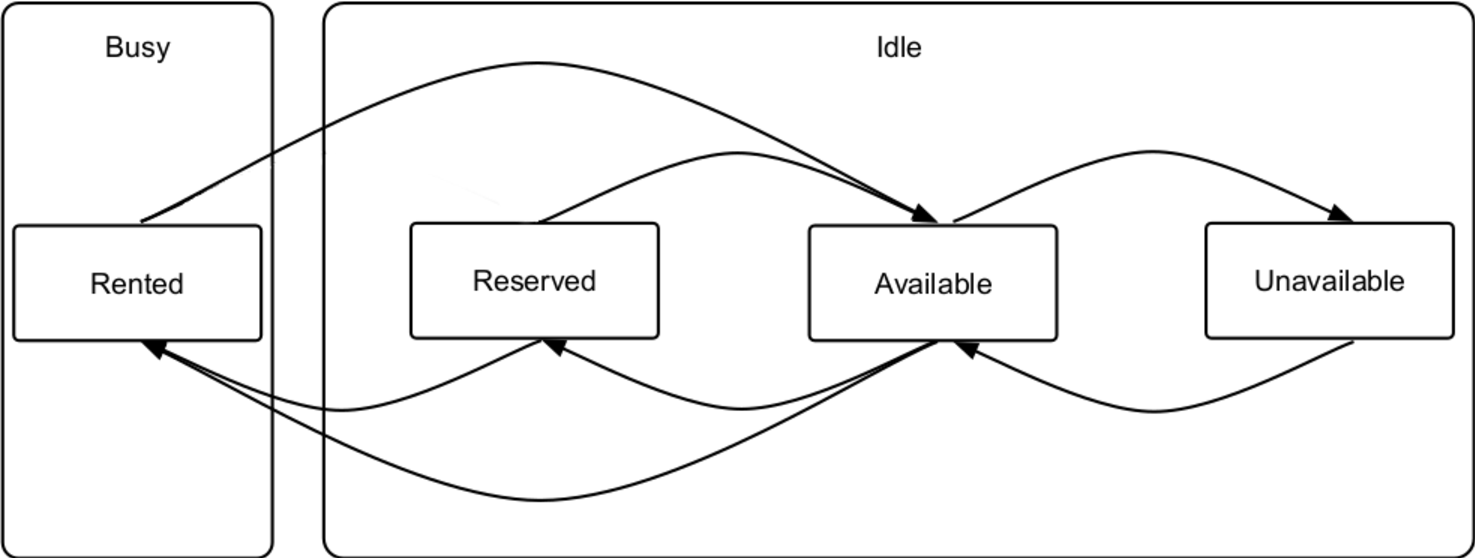
\includegraphics[width=1\textwidth]{imagens/diagrama_v4.pdf}
\caption{Possible states of a vehicle in a car-sharing system.}
\label{fig:diagrama}
\end{figure}

\section{Datasets and crawling methodology} 
\label{sec:3_4_methodology}

%FLEET OF CS systems
Our work relies on usage data from three car-sharing services: Modo, Car2Go, and Evo. These services operate in several cities and countries. We focus on data from the Vancouver area, where all these three services operate. Modo fleet is composed of combustion, electric and hybrid cars; Car2go offers combustion cars and finally, Evo supplies only hybrid vehicles. For each service, we collected both users' trips and fleets composition. In total, we observed more than 680 cars for Modo, 1\,200 for Car2go, and 1\,000 for Evo.

% DATA COLLECTION
For all the three services, we collected vehicle status minute-by-minute, through public Application Programming Interfaces (APIs) or, directing accessing their service information web-page. We can get some values like vehicle ID and position.  In short, through the Modo API\footnote{Modo API, \url{http://modo.coop/api/}} we can obtain the station of a vehicle and the period it is available, reserved or running.
The data we get from Evo\footnote{Evo public portal, \url{https://www.evo.ca/api/Cars.aspx}} information page allow us to check the remaining fuel  (in percentage) of a vehicle and its location. Finally, Car2go APIs\footnote{Car2go API, \url{https://www.car2go.com/api/tou.htm }} output is similar to the Evo's one. 
Data from Evo and Modo comprises five months, ranging from March 1st, 2018 to July 16th, 2018. Car2Go data comprises thirteen months, ranging from  December 31st, 2016 to January 31st, 2018. It is important to notice that, to not violate the users' privacy, the providers do not expose any users' personal information. Moreover, the companies do not track the cars during a trip so we do not know exactly the travel path, but only the start/end positions and the duration of travel.

All measurements used in our analyses are publicly available the following trace repository:
\url{http://netlab.ice.ufjf.br/index.php/carsharingdata/}

%In the following, we further explain each service crawling methodology and the data we use in our analysis.

%In Modo, we infer the reservation period by the availability intervals and the minute-by-minute collect, whereas Evo and Car2Go data allow us to exactly trigger the moments in which the users begin and over their trips, with a precision of one minute, just monitoring the state of all cars. 


\subsection{Modo crawling methodology and data summary}


%%%%%%%%%%%%%%%%%%%%%%%%%%%%%%%%%%%%%%%%%%%%%%%%%%5

%MODO data collection
The Modo data collection process was conducted with a crawler that uses its public API. 
First, we request to the Modo API the list of all vehicles of the service. 
Then, minute by minute, we request the status of each of these vehicles. Each request returns the schedule of a vehicle, informing the periods it will be available for the next 24-hours. Moreover, it returns the vehicle location, i.e., the station with its identifier. 
Note that Modo API does not return specific vehicle status, nor any information that could be used to identify users of the system. We uncover if a vehicle is busy or idle based on its reservation period and the current observation time. In other words, we collect several vehicle schedules and compare each other.
Figure~\ref{fig:capturas} illustrates the process of collecting data for a given vehicle. Each data sample corresponds to a request to the API in the order they occur. Data sample \#1 is the result of the API request at minute 1 ($t=1$), data sample \#2 is the result of the API request at minute 2 ($t=2$), etc. At each data sample, the blue dot represents the time a vehicle will be available. We highlight three possible situations:

\begin{itemize}
\item First, as shown in Figure~\ref{fig:capturas}(a), at $t=1$ a given vehicle is shown reserved up to $t=5$.  At $t=2$, the new request to the Modo API still show us that the vehicle will be available only at $t=5$. Each of the following requests to the API confirms the booking period. At the time $t=6$, we perform a request to the API and the vehicle is no longer booked. In sum, we are able to infer that someone booked the vehicle before or at $t=1$, and returned it to the station at $t=5$.

\item Second, as shown in Figure~\ref{fig:capturas}(b), at $t=1$  the Modo API returns that a given vehicle is reserved up to $t=6$.  However, in this case, a request at $t=5$ shows the vehicle is no longer reserved. In this case, we can infer that the user returned the vehicle earlier to the station which means she/he used the vehicle only up to $t=5$.

\item Finally, as shown in Figure~\ref{fig:capturas}(c), the user may extend the booking period. More precisely, at $t=1$ the given vehicle is reserved up to $t=5$. At the third request, we note that the vehicle will no longer be available at $t=5$ but $t=6$. The following API requests confirm the use of the car until $t=6$.
\end{itemize}


\begin{figure}[!htb]
\centering
    \begin{minipage}[b]{0.25\linewidth}
      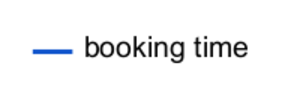
\includegraphics[height=0.8cm]{modo_methodology/time.pdf}
    \end{minipage}\hspace{-5mm}
    \begin{minipage}[b]{0.25\linewidth}
      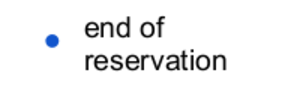
\includegraphics[height=0.8cm]{modo_methodology/point.pdf}
    \end{minipage}

    \medskip
    \begin{minipage}[b]{0.32\linewidth}
    \centering
     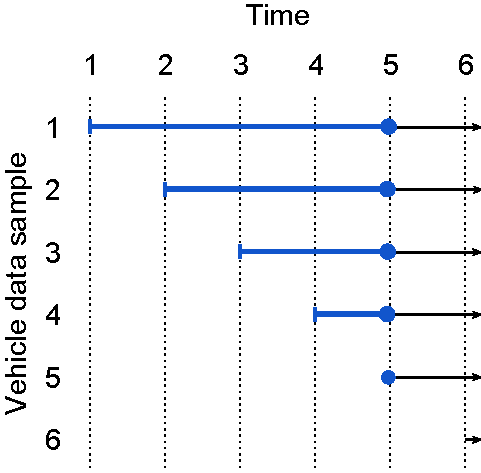
\includegraphics[width=30mm]{modo_methodology/Normal_Situation.pdf}
     {\\(a) Normal \\situation}
    \end{minipage}
    % \hspace{5mm}
    \begin{minipage}[b]{0.32\linewidth}
     \centering
     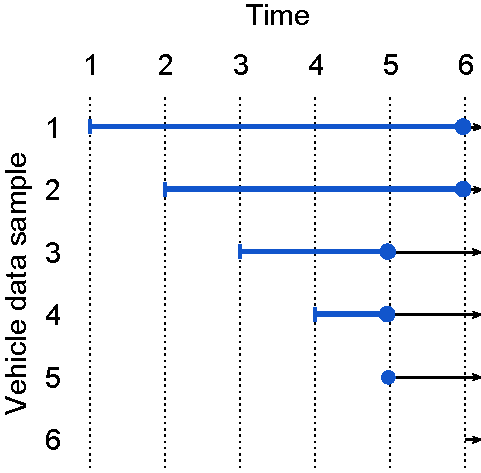
\includegraphics[width=30mm]{modo_methodology/Cancelation_Situation.pdf}
    %  \vspace*{-3mm}
     {\\(b) Anticipated vehicle return}
    \end{minipage}
    %\hspace{1cm}
    %\hspace{5mm}
    \begin{minipage}[b]{0.32\linewidth}
    % \vspace{5mm}
     \centering
     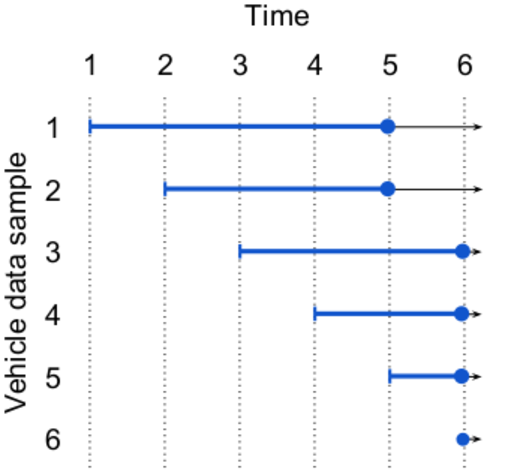
\includegraphics[width=30mm]{modo_methodology/Consecutive_without_legend.pdf}
     {\\(c) Extended travel situation}
    \end{minipage}
    \caption{Possible vehicle status during the Modo crawling. In (a) a normal booking and usage situation; (b) a cancellation situation; (c) a consecutive booking situation.}
    \label{fig:capturas}
\end{figure}

Besides, we also collect base stations location, vehicle models and whether the vehicle is electric or hybrid. 
Table~\ref{table:dataModo} summarizes the data we have collected from Modo. We stored 134 millions of records in 5 months, from a fleet of 682 vehicles distributed in 528 stations, each of them with one or more cars. The stations are located in Vancouver, Canada, and its neighbor cities. This data allows us to analyze more than %149 thousands of booking records and 
98\,000 travels.\footnote{Data are available on http://netlab.ice.ufjf.br/index.php/carsharingdata/}
% \footnote{Data will be available for researchers upon request.}

\begin{table}[tbh]
\centering
\scriptsize
\begin{tabular}{llr}
%\multicolumn{2}{l}{Description}                     & Amount \\ 
\hline
\multicolumn{2}{l}{\# of Collected Records}  & $\approx$ 134\,000\,000\\
\multicolumn{2}{l}{\# of Booking Records} & 149\,732  \\
\multicolumn{2}{l}{\# of Travels Records} & 98\,915   \\
\multicolumn{2}{l}{\# of Stations} & 528    \\\hline   
\multirow{3}{*}{\# of Vehicles}       & - Common    & 530 \\
                                      & - Hybrids  & 148 \\
                                      & - Electrical & 4 \\
                                      \hline
\end{tabular}
\caption{Summary of the Modo dataset.}
\label{table:dataModo}
\end{table}


%%%%%%%%%%%%%%%%%%%%%%%%%%%%%%%%%%%%%%%%%%%%%%%

\subsection{Evo crawling methodology and data summary}

Evo does not offer a public API to researchers. For this reason, we collect data which is publicly available at its web portal. Minute by minute, we retrieve a list of all system vehicles. Moreover, we request service snapshots, describing which vehicles are parked, where they are parked and if they are available to travel. 
We process all snapshots of the system to infer the moments a vehicle is busy (rented) or idle (parked at a station). During a snapshot, if a vehicle is listed among the system vehicles but it is not parked at any station, we infer it is in use. Then, we set-up the travel starting point as the last station the vehicle was parked. Analogously, the travel ending point will be the next station the vehicle appears in a future snapshot. The total travel time is accounted for as the difference between these snapshots times. 
For each travel we identify, we also record the end-to-end path, according to the Google Maps API. In this way, we are also able to calculate the estimated travel, taking into account the local traffic conditions. Clearly, this estimation does not take into account the car-sharing client behavior and, as a consequence, differ from the real travel time we also store. 
One may reserve a car in Evo and cancel this reservation, within a thirty minutes range, without any charges. Thus, we infer the number of cancellation in Evo by filtering short travels (i.e., $<$ 30 minutes) where the start and end points are the same. To accommodate GPS imprecision, we consider a 3~meters threshold. 
Table~\ref{table:dataEvo} summarizes the data we collect from Evo.
%In short, we collected more than 10 million records and 1 million travels, of a fleet with more than a one thousand vehicles and 130 stations. 
Note that this service does not need a large number of stations because the user can park the car in some public park spots in the service area, that is called home zone (Vancouver and its neighbor cities).

\begin{table}[htb]
\centering
\scriptsize

\begin{tabular}{llr}
%\multicolumn{2}{l}{Description} & Amount\\ 
\hline
\multicolumn{2}{l}{\# of Collected Records} & 142\,853\,500
\\
\multicolumn{2}{l}{\# of Travels Records} &  644\,887\\
%1\,232\,262\\
\multicolumn{2}{l}{\# of Stations}  & 130  \\\hline
\multicolumn{2}{l}{\# of Vehicles} & 1\,237
%1\,003 
\\\hline
\end{tabular}
\caption{Summary of the Evo data collection.}
\label{table:dataEvo}
\end{table}

\subsection{Car2Go crawling methodology and data summary}

Car2Go offers APIs providing information about available cars at the moment of the request. Each API request returns, among other information, the car unique ID, its position and other fields which specifically describe the car status. Therefore the API response is semantically equivalent to the Evo's one. In this way, we applied the same methodology to gather and store the Car2go data too.

There are two main events, which changes the car status, clearly observable from the data. Considering the current time instant $t_i$: 
\begin{itemize}
     \item if in $t_i$ the car is present in the API response and at time $t_{i+1}$ it is not, that car passes from available to rented. %It represents a parking event finish and a booking.
     \item if in $t_i$ the car is \emph{not} present and at time $t_{i+1}$ it reappears in the API reply, that car passes from rented  to available. It represents a booking finish and a parking beginning.  Indeed, for privacy constraints, the position of the car during a booking is not available.
\end{itemize}

Notice that from a single rented status is impossible to estimate the traveled distance: by computing the Euclidean or Haversine 
distance we obtain only a lower bound of the real travel distance which is practically too optimistic to be used as a primary travel estimation. To improve this estimation we attach to each entry the distance provided by the Google Maps API. 
As in Evo's methodology, we infer the number of cancellations by filtering short travels where the start and end points are very close. Table~\ref{table:dataCar2Go} summarizes Car2go dataset. We have more than one million travels in our thirteen months of data. As a free-floating service, Car2Go does not have stations but it has an operation zone, that covers a large area of Vancouver city and North-Vancouver. 

\begin{table}[htb]
\centering
\scriptsize
\begin{tabular}{llr}
%\multicolumn{2}{l}{Description} & Amount\\ 
\hline
\multicolumn{2}{l}{\# of Travels Records} & 1\,095\,577\\
%1\,340\,053\\
\multicolumn{2}{l}{\# of Vehicles} & 1\,077
%1\.273 
\\\hline
\end{tabular}
\caption{Summary of the Car2Go data collection.}
\label{table:dataCar2Go}
\end{table}

\section{Temporal Analyses}
\label{sec:results}

In this section I show different analysis to discover and characterize how the FFCS are used. In the first part of the section, I analyse the temporal systems characterization to understand if FFCS are actually used and when.

I consider a period from December 10th 2016 to January 31st 2017, the first reliable collected data chunk. The system observed 125,000 snapshots, about 104,000 bookings for car2go and 93,000 for Enjoy. In Turin, the fleet of car2go was composed by 394 cars, and the fleet of Enjoy was composed by 172 cars.

In order to make clear the rest of the book, it necessary to univocally define the basilar entities related to the car status in the data lake defined in the chapter \ref{chap:2_dataset}, section \ref{sec:2_4_data_normalization}.

\begin{definition}{the \textbf{Parking}}
	\label{def:parking} is the time period in which the car is present in, at least, two consecutive snapshot. Therefore that car it is available for an user reservation
\end{definition}
\begin{definition}{the \textbf{Booking}}
	\label{def:booking} is the time period in which the car is NOT present in, at least, two consecutive snapshot. There fore an user booked that vehicle or the provider temporary removed it for maintenance.
\end{definition}


\subsection{System Utilization}

\begin{figure}
\centering
 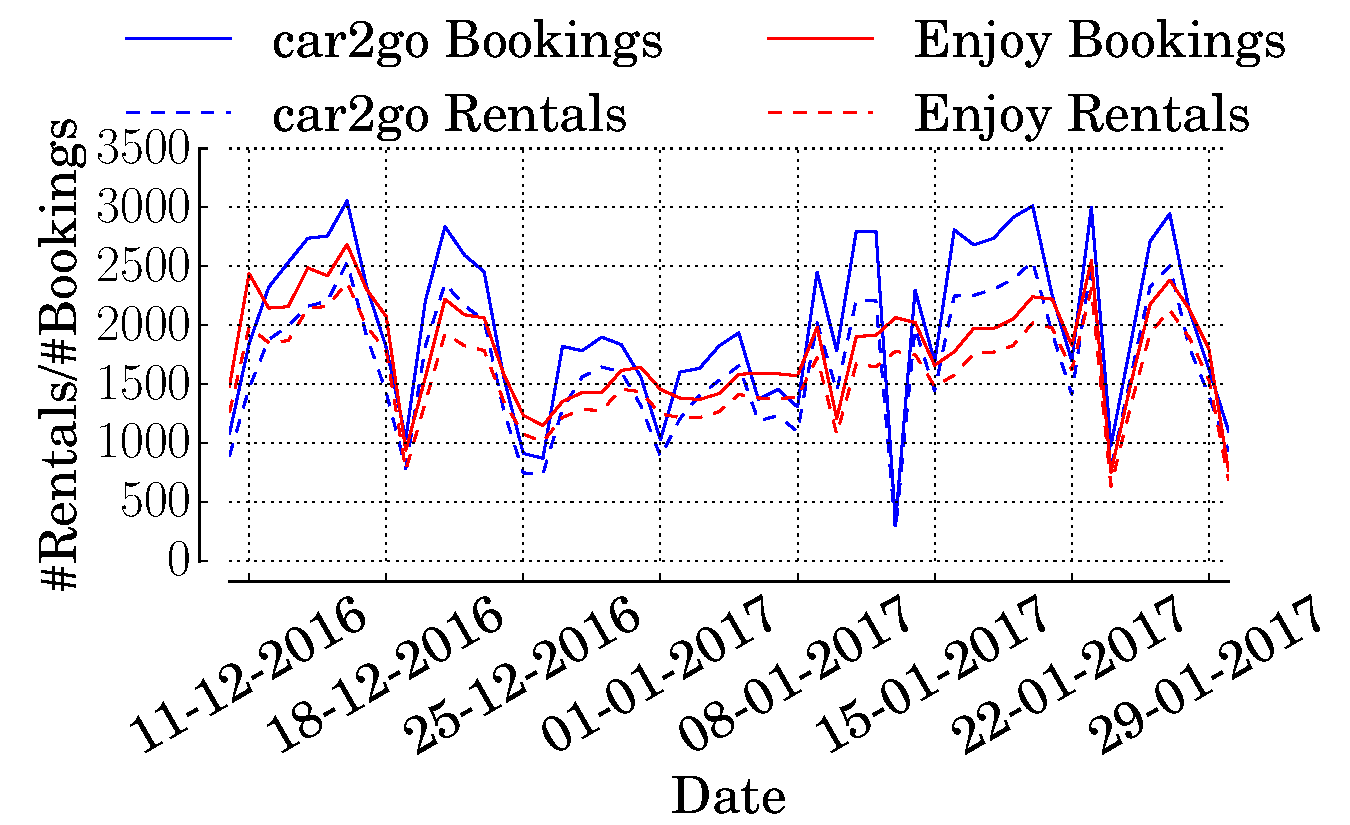
\includegraphics[width=0.85\columnwidth]{figures/bookings.pdf}
 \caption{Total number of bookings and of rentals per day for car2go and for Enjoy \label{fig:bookings}}
\end{figure}
The providers, in this case study, allows the users to \textit{reserve} a car before the ride. More in details, the provider makes the reserved car unavailable for the other users without billing the customer who reserved the car. When the reservation time (that changes for each provider), the billing mechanism starts even if the engine it is still off. The customer can cancel the reservation without any expense if it happens before the reservation time. With this mechanism, the providers would let the possibility to the users to reach the cars by foot.

Given that, it is now possible to the define:
\begin{definition}{\textbf{Reservation}}
	\label{def:reservation} A reservation it is a booking where the initial and final destination matches and the duration is lower than the provider's reservation time.
\end{definition}

\begin{definition}{\textbf{Rental}}
	\label{def:rental} A rental it is a booking where the initial and final destination are different.
\end{definition}


Starting from December 10th, Figure~\ref{fig:bookings} plots the total number of bookings and the total number of rentals recorded on each day, for car2go (blue curves), and for Enjoy (red curves). Obviously, being the latter a subset of the first, its number is always smaller. However, during some days, the discrepancy is well visible; that means that the operation of booking cancellation is not so rare.

Interestingly, firstly, both car2go and Enjoy follow a similar behaviour with the number of bookings and rentals decreasing in the Christmas period and increasing again after the Epiphany. 

Secondly, despite car2go fleet has more than twice as much cars than Enjoy (394 vs. 172), the number of car2go bookings does not show such a higher value with respect to Enjoy. With Enjoy having more bookings in some snapshots e.g., December 10th and 11th. Moreover, in some points (ecember 19th, January 24th) it is possible to detect huge drop due to the failure of our crawler. 

Moreover, some drops in bookings' values are noticeable. Those sudden changes can be addressed to some failures, in the crawlers (e.g., when all curves suddenly drop) or in the operators' web services(e.g., when only one system suffers a sudden drop).



\begin{figure}
\centering
 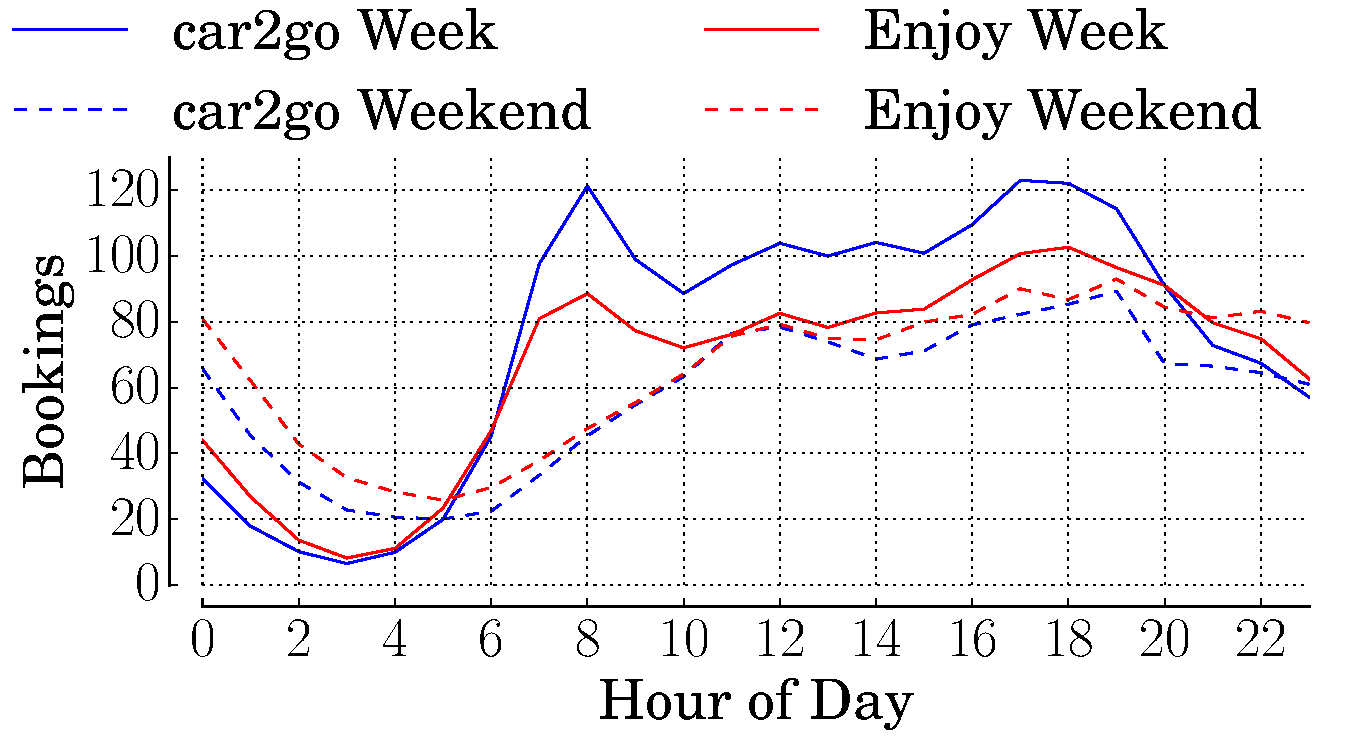
\includegraphics[width=0.85\columnwidth]{figures/bookings_day.pdf}
 \caption{Mean number of bookings in weekdays and weekends for car2go and Enjoy\label{fig:bookingsweek}}
\end{figure}

Looking at the data with a finer granularity, it is noticeable that the car sharing adoption changes during the day. To better characterize this, I separate weekdays and weekends. The figure~\ref{fig:bookingsweek} points out the trend over the day. The curves report the average number of bookings over the entire period  in each hour of the day.

Firstly, it is possible to see that weekdays and weekends have a quite different trend. During the weekend FFCS systems are more used at night with respect than weekdays, with on average at midnight of 80 and 60 bookings per hour for Enjoy and car2go. Instead, the figure shows how during the weekdays both car2go and Enjoy have their peak of usage at 8~am and between 5~pm and 7~pm. This trend can be easily explained as, during that time slots, FFCS customers use cars to go and return from work. 
As previously indicated, despite car2go has twice the number of cars than Enjoy, the system utilization of the latter is higher, with peak utilization topping to 60\%, versus 30\% of car2go. 

Even in absolute number of rentals, Enjoy shows an higher number of bookings after 8~pm during the weekdays, and always during the weekends. This can be explained by the car models adopted by the two companies. While car2go uses the compact-two seats \textit{Smart}, Enjoy fleet is composed of \textit{Fiat 500}, which are 4 seats cars. Rentals prices are instead comparable (0.24\euro/min Enjoy vs 0.25\euro/min car2go). Data suggests that Enjoy looks more appealing during the times when people prefer to share the ride, and during weekends when families and groups move. 



\section{Rides Characterization}
In this section, I give a detailed look about driving habits. In particular I compare driving distances and duration of rentals and parking duration. Finally I conclude with some insights about the variation of spatial demand, characterizing which and because some zones attract or generate more rentals with compared to other one.


\subsection{Driving patterns}


%\begin{figure}[t!]
%	\centering     %%% not \center
%	\subfloat[][ECDF of the booking duration when the booking does not produce a rental. Weekdays and weekends]
%	{\label{fig:3_5_pdf_norent}
%		\includegraphics[width=0.33\columnwidth]
%		{figures/no_rent.pdf}
%	}
%	\subfloat[][ECDF of the rental duration. Weekdays and weekends]{\label{fig:3_5_cdf_duration}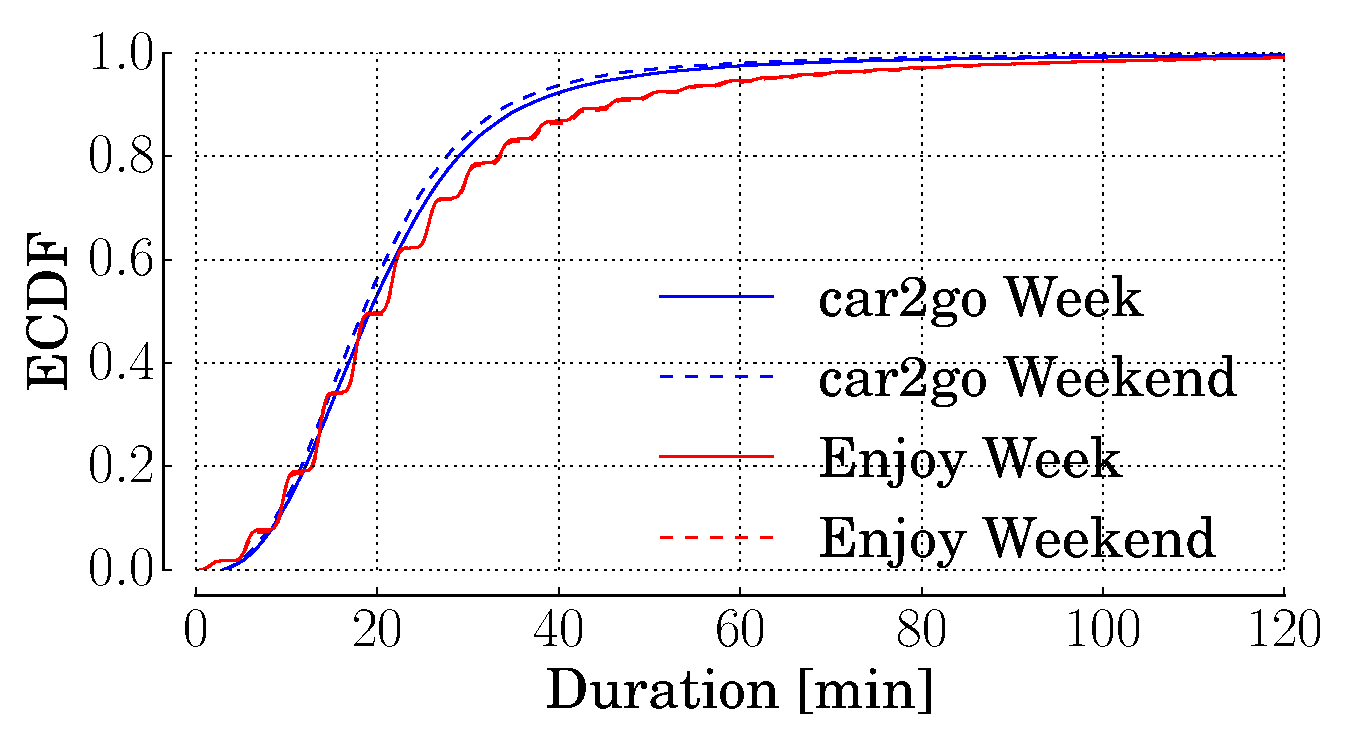
\includegraphics[width=0.33\columnwidth]{figures/duration.pdf}}
%	\subfloat[][ECDF of the rental distance. Weekdays and weekends]{\label{fig:3_5_cdf_distance}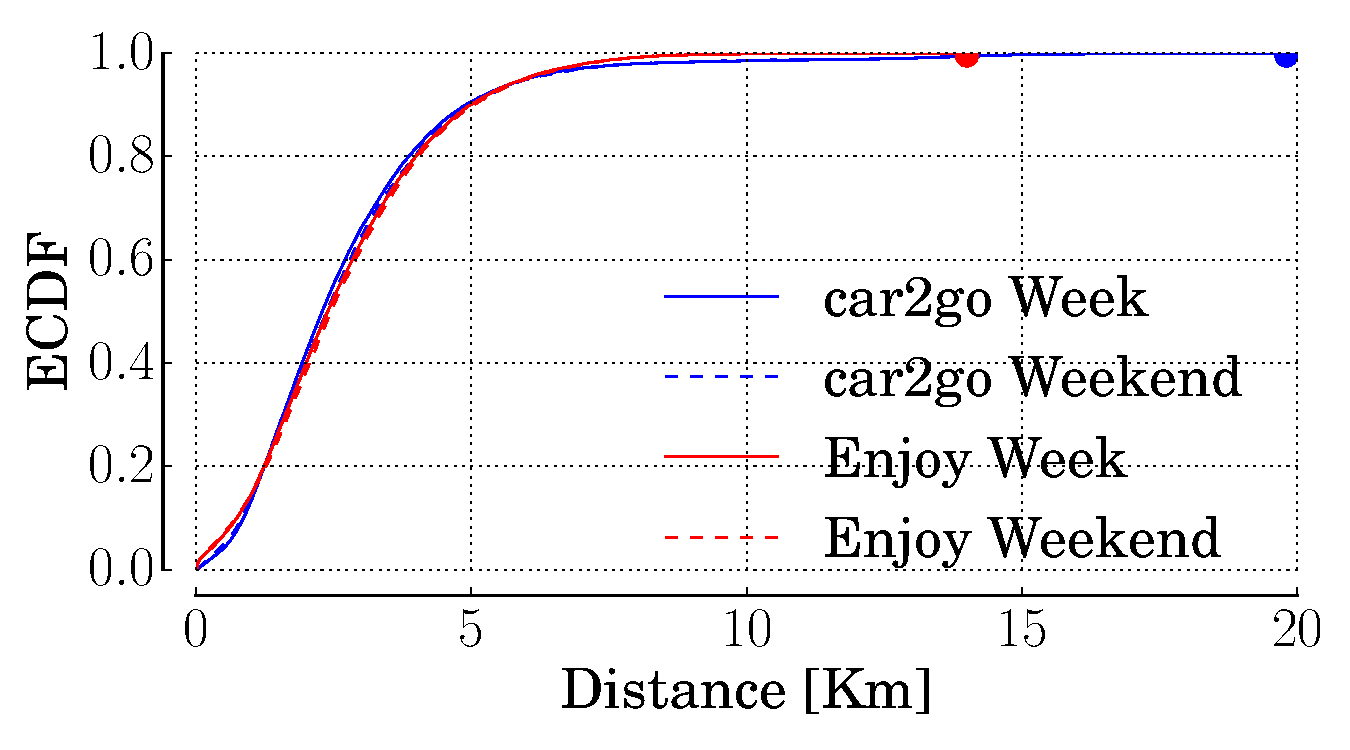
\includegraphics[width=0.33\columnwidth]{figures/distance.pdf}}
%	\caption{Users' booking and rentals habits \mc{magari immagini singole}}
%	\vspace{-3pt}
%\end{figure}


Now, I show how users tend to use FFCS systems during weekdays and weekends. I study three different aspects of users' behaviour: 
\begin{itemize}
	\item for how long users reserve the car before cancelling a booking (Figure~\ref{fig:3_5_pdf_norent})
	\item for how long users rent a car (Figure~\ref{fig:3_5_cdf_duration})
	\item how far users drive (Figure~\ref{fig:3_5_cdf_distance})
\end{itemize}

\begin{figure}
	\centering
	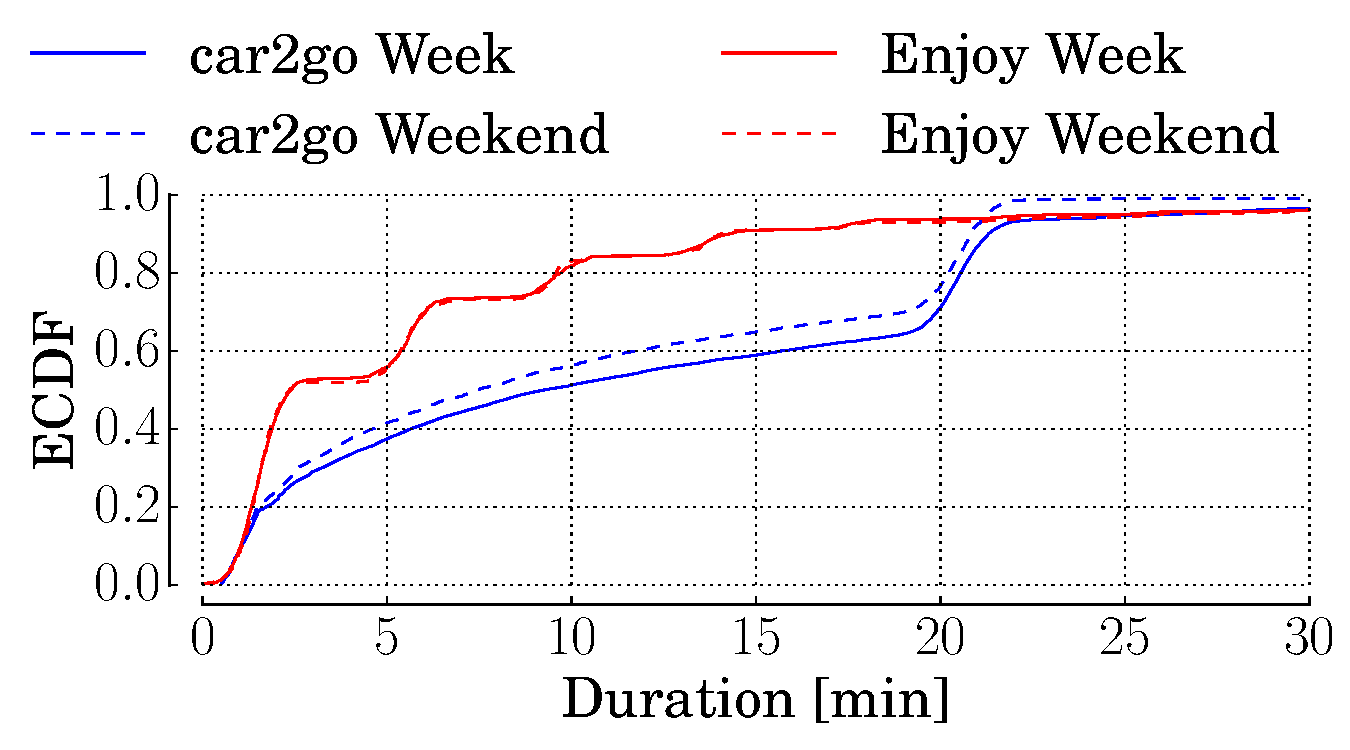
\includegraphics[width=0.85\columnwidth]{figures/no_rent.pdf}
	\caption{ECDF of the booking duration when the booking does not produce a rental. Weekdays and weekends \label{fig:3_5_pdf_norent}}
\end{figure}

First, I check if and for how long users reserve a car and then they cancel a booking. Interestingly, only a small subset of Enjoy bookings are affected by cancellation with respect to car2go bookings. In particular, the dataset presents 14.9\% of car2go and 2.9\% of Enjoy bookings cancellation. This again hints for people preferring to use the Fiat 500 offered by Enjoy, so that they hardly cancel a booking when they reserved an available vehicle. On the contrary car2go availability is higher and so it looks easier to find a closer car. People may thus cancel a previous booking when they find a closer vehicle. Another hypothesis is that car2go may be used as a ``backup'' until an Enjoy vehicle becomes free in the user's area. 

Looking at when people cancel the reservation, figure~\ref{fig:3_5_pdf_norent} shows the CDF of reservation time. Indeed, car2go tends to have a smaller percentage of cancellation within 5 minutes, with a huge step at about 20 minutes. While the first ramp can be explained as a communication error or as some sudden cancellation, the latter can be explained by the \textit{maximum free-of-charge reservation time} of car2go. Truly, users, may reserve a car up to 20 minutes without paying any fee. The same trend is not present for Enjoy which offers a \textit{maximum free-of-charge reservation time} of 15 minutes. Instead, the curve shows a peak at 2 minutes and then a decreasing trend after 15 minutes, when almost all the cancellation are already done.
One last important aspect that this picture shows is how the Enjoy curves have some steps instead of being smooth as the car2go ones. 
This hints to periodic updates on web system so that a time granularity emerges.
To shed some lights on this phenomenon, I performed some active experiments with the Enjoy web portal. The experiment consists of making a new reservation and find when our crawler detects that the car actually disappears from the set of available cars. Then, as soon as I spot the car disappearing, I cancel the reservation to detect when the car reappears in the system. Surprisingly, I discover that when we make the reservation, the car immediately disappears from the system, instead, when I cancel the reservation, the system takes between 1 and 4 minutes to actually show the car again. The presence of such an offset causes the steps in the Enjoy curves which are affected by an artificial delay. To take into account this offset all Enjoy duration have been decreased of 2.5 minutes, i.e., the average delay the Enjoy system adds. 


\begin{figure}
	\centering
	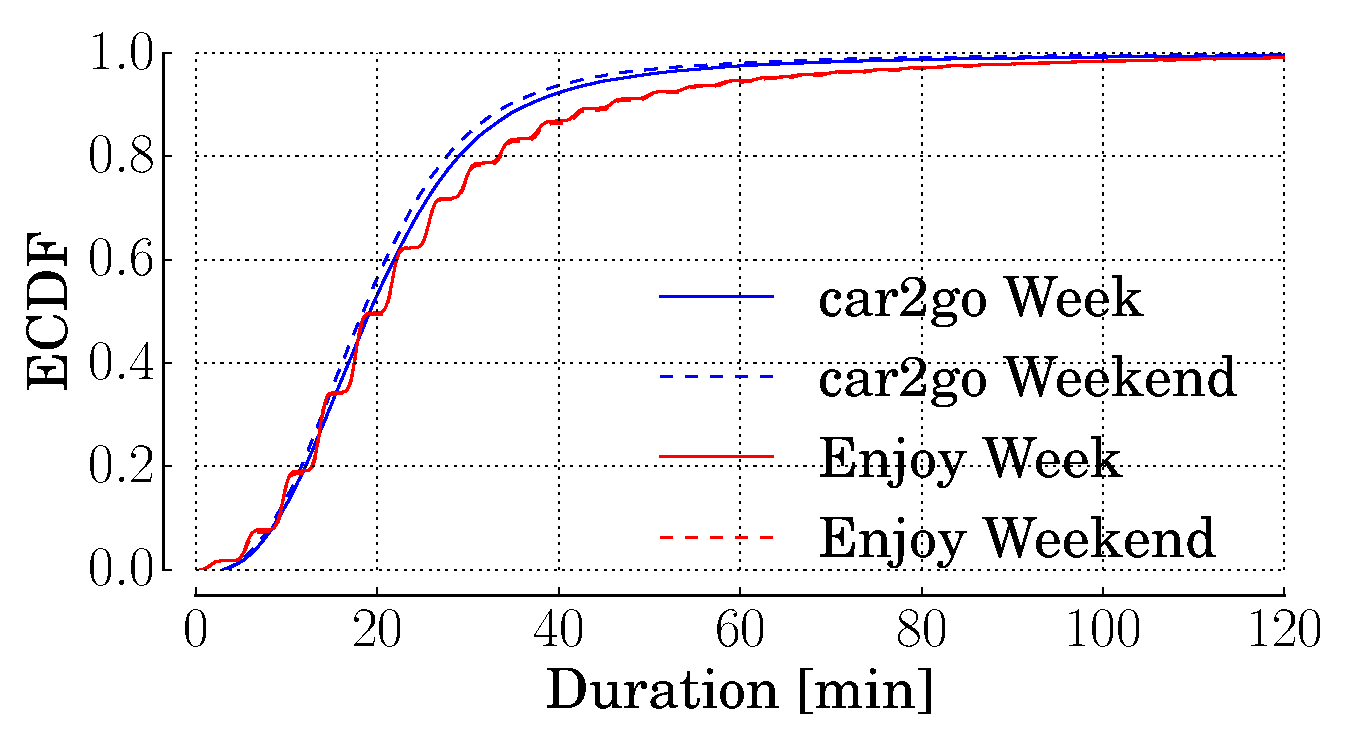
\includegraphics[width=0.85\columnwidth]{figures/duration.pdf}
	\caption{ECDF of the rental duration. Weekdays and weekends\label{fig:3_5_cdf_duration}}
\end{figure}


I next move to characterize the rental duration. Figure~\ref{fig:3_5_cdf_duration} depicts the Empirical Cumulative Distribution Function (ECDF) of the booking duration for Enjoy and car2go during the weekdays and the weekends. The plot shows how the trend tends to be equal during the weekdays and the weekends. This demonstrates that, despite the different pattern of utilization shown before, the booking duration time results similar. Secondly, the ECDFs of car2go and Enjoy are almost overlapped, highlighting how these two services tend to be used in a similar way. Indeed, most of the rentals last less than 1 hour, with 80\% of them lasting less then 30 minutes. It is important to remark that this times include also the reservation time, i.e., the time the user can reserve a car for free before driving it, and the time to find a parking place. Therefore the actual driving time may be significantly smaller.


\begin{figure}
	\centering
	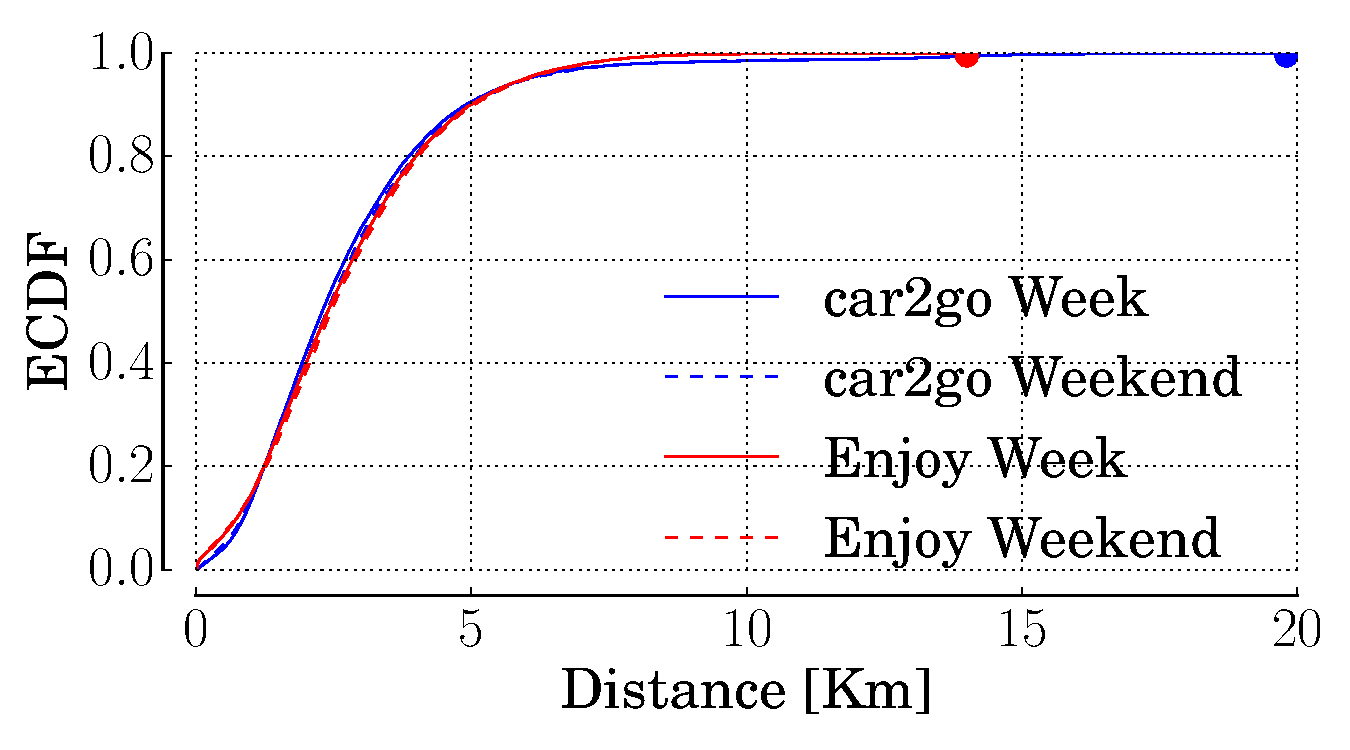
\includegraphics[width=0.85\columnwidth]{figures/distance.pdf}
	\caption{ECDF of the rental driven distance. Weekdays and weekends\label{fig:3_5_cdf_distance}}
\end{figure}


I repeat the same analysis considering the driving distance as reported in Figure~\ref{fig:3_5_cdf_distance}.
To determine the driving distance of each trip we exploit the Google Direction APIs to get the shortest path from the origin to the destination. Similarly, for the driving duration, car2go and Enjoy show a comparable behaviour, and marginal changes during weekdays and weekends. Interestingly, the graphs points out that the 90\% of the trips last less then 5~km demonstrating that most of the rentals are used for short trips both in term of time, and in term of distance. Lastly, the car2go curves saturate many km later than the Enjoy ones as highlighted by the circles. This is due to the possibility to reach the airport of Turin with the car2go cars, which is about 20 km far. 



\begin{figure}[t!]
\centering
\vspace{-10pt}
 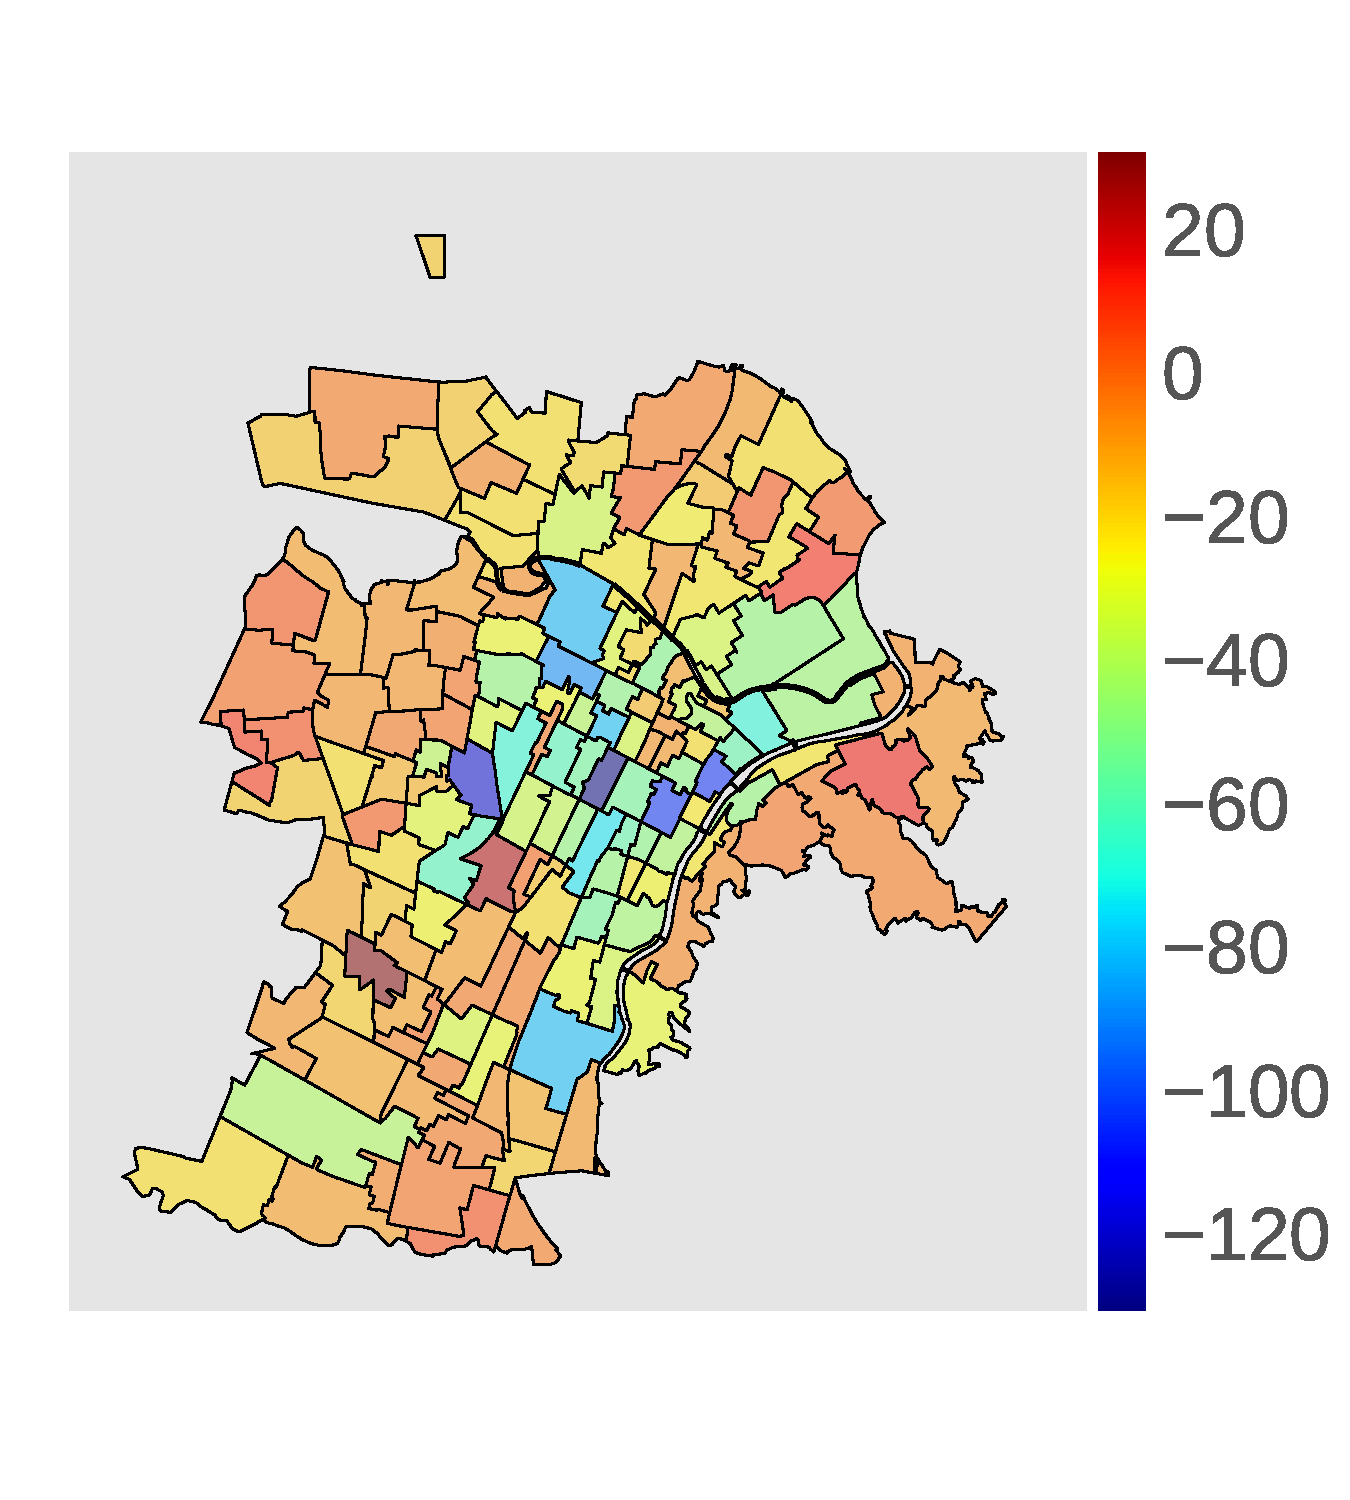
\includegraphics[width=0.72\columnwidth]{figures/clorophlet_o_minus_o1.pdf}
 \vspace{-10pt}
 \caption{Heatmap of arrival - departure per area from 7~am to 12~am vs from 5~pm to 9~pm \label{fig:3_5_heatmap_arr_dep}}
\end{figure}


\subsection{Spatial Analysis}  


In the previous section I analysed car2go and Enjoy only from a temporal point of view. In order to have a complete scenario, it is necessary to study recurrent spatial patterns. To do that I projected the initial and final coordinates on the Turin's neighbour map. Then I computed the attractiveness of each neighbour. Figure~\ref{fig:3_5_heatmap_arr_dep} shows the attractiveness of the  zones in Turin by analyzing the departure and arrival zones. For each zone I compute the difference between bookings ended in the evening [5~pm - 9~pm] and bookings ended in the morning [7~am, 12~am]. Red {areas are those} more attractive during the evening, while blue areas are more attractive in the morning. It is clear that the city center is the most popular destination for car sharing during the office hours, while the trips are sparsely ending in the suburbs during the evening.


\subsection{Users' Habits}

I now characterize how users drive and what is the correlation between public transport usage and availability.

To observe users' driving habits, I use the \textit{driving time} returned by the Google Directions APIs to {obtain} the estimated {driving} time from {rental initial position to the rental final position}. Intuitively, the {rental} time is longer than the driving time as it takes into account also the {reservation} time, and the time to find a final parking spot. Figure~\ref{fig:3_5_heatmap_driving} shows an heat map where the X axis represents the Google estimated driving time and the Y axis the actual booking time. Each cell counts the number of {observed} trips {for each (x,y) pairs}.
For the ease of representation the values are rounded by minute. The diagonal line separates the area where the booking time is lower/greater than the driving time. As expected, most of the trip falls in the area where the booking time is greater then the driving time. However, a non negligible number of trips (12.1\%) falls in the area where the booking time lasts less than the driving time. 

\begin{figure}[h!]
	\centering
	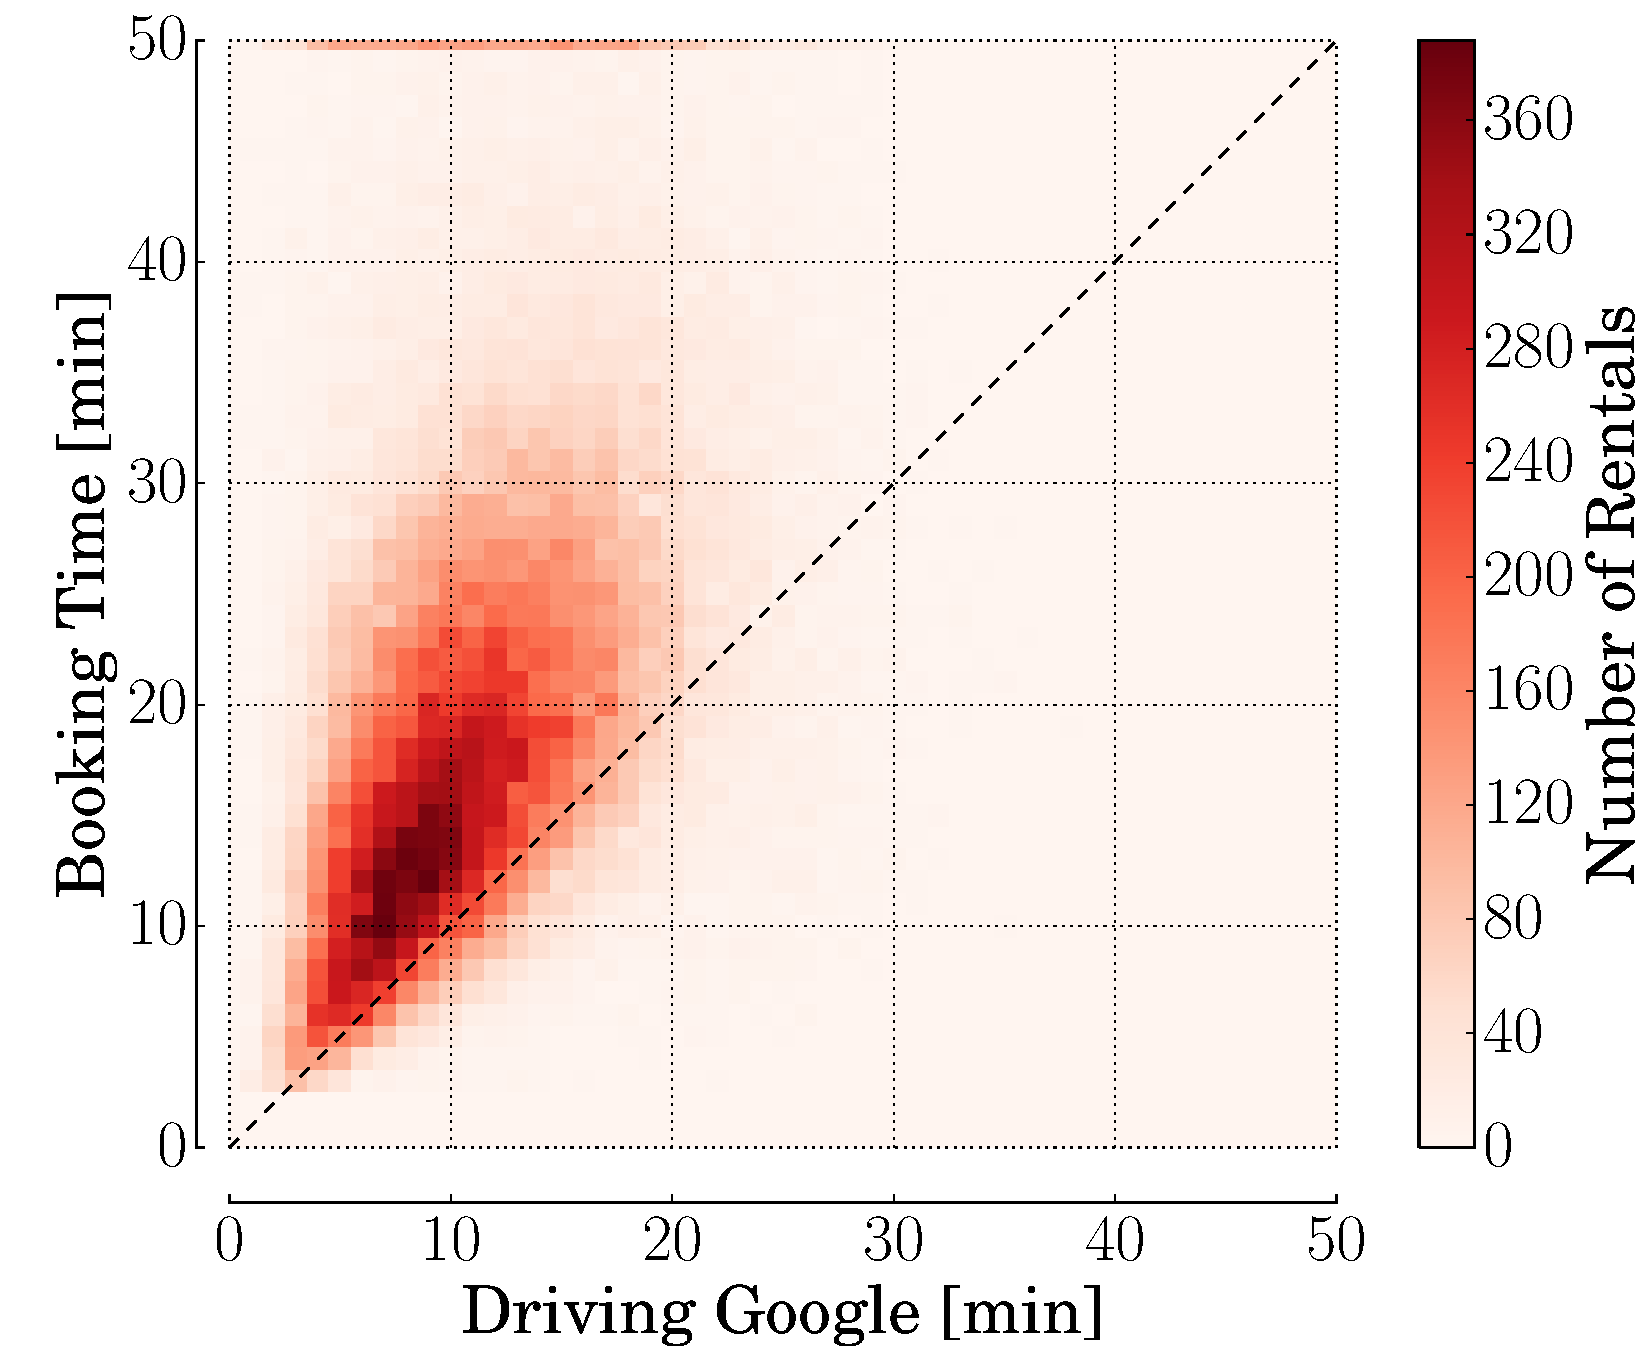
\includegraphics[width=0.85\columnwidth]{figures/car2go_faster_driving.pdf}
	\caption{Heatmap of booking time vs estimated driving time by Google\label{fig:3_5_heatmap_driving}}
\end{figure}


This may be due to several factors: Google Directions possibly overestimating the average trip duration, or users driving faster than expected.
To better quantify how much faster users drive the car in those cases, I  computed the difference between the driving time and the actual booking time. I show the Empirical Cumulative Distribution Function of such values in Figure~\ref{fig:3_5_cdf_faster_google}. It is possible to see that te most of these trips are only 5 minutes faster than the estimated driving time, with Enjoy users which seems to drive faster than car2go ones. Indeed, if the trip is more than 10 minutes faster, Google suggested a longer path to the destination, e.g., suggesting to take the highway which was much longer with respect to crossing part of the city.

This analysis hints that the current pricing policy, which depends only by the booking time, may have some drawbacks as it may encourage users to drive fast. An hybrid pricing policy, which takes into account both the time and the distance, may be effective in solving this problem, e.g., by increasing the price in case of an user drive faster than expected, or by reducing the fee in case of traffic congestion.

\begin{figure}[h!]
	\centering
	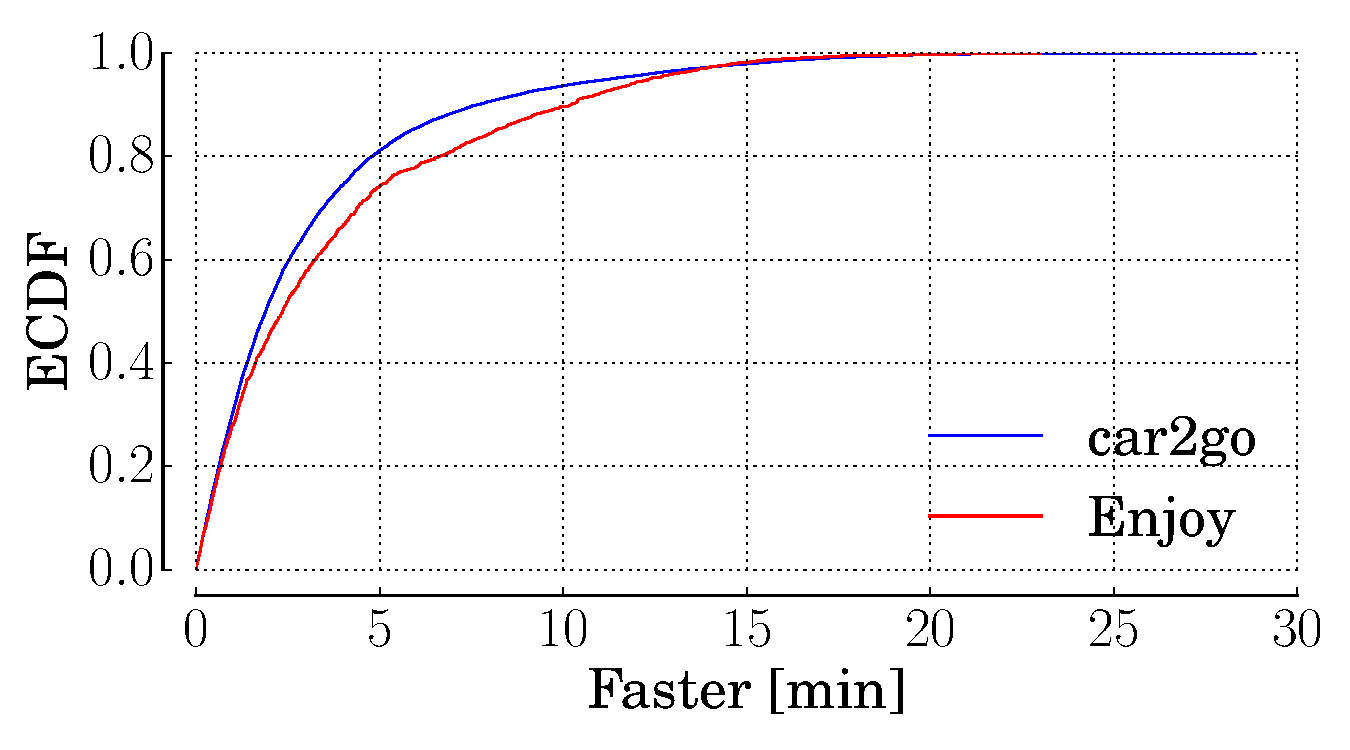
\includegraphics[width=0.85\columnwidth]{figures/faster_driving.pdf}
	\caption{ECDF of the difference between the expected driving time and the actual driving time\label{fig:3_5_cdf_faster_google}}
\end{figure}


%\begin{figure}[t!]
%\centering     %%% not \center
%\subfloat[][Heatmap of booking time vs estimated driving time by Google]{\label{fig:heatmap_driving}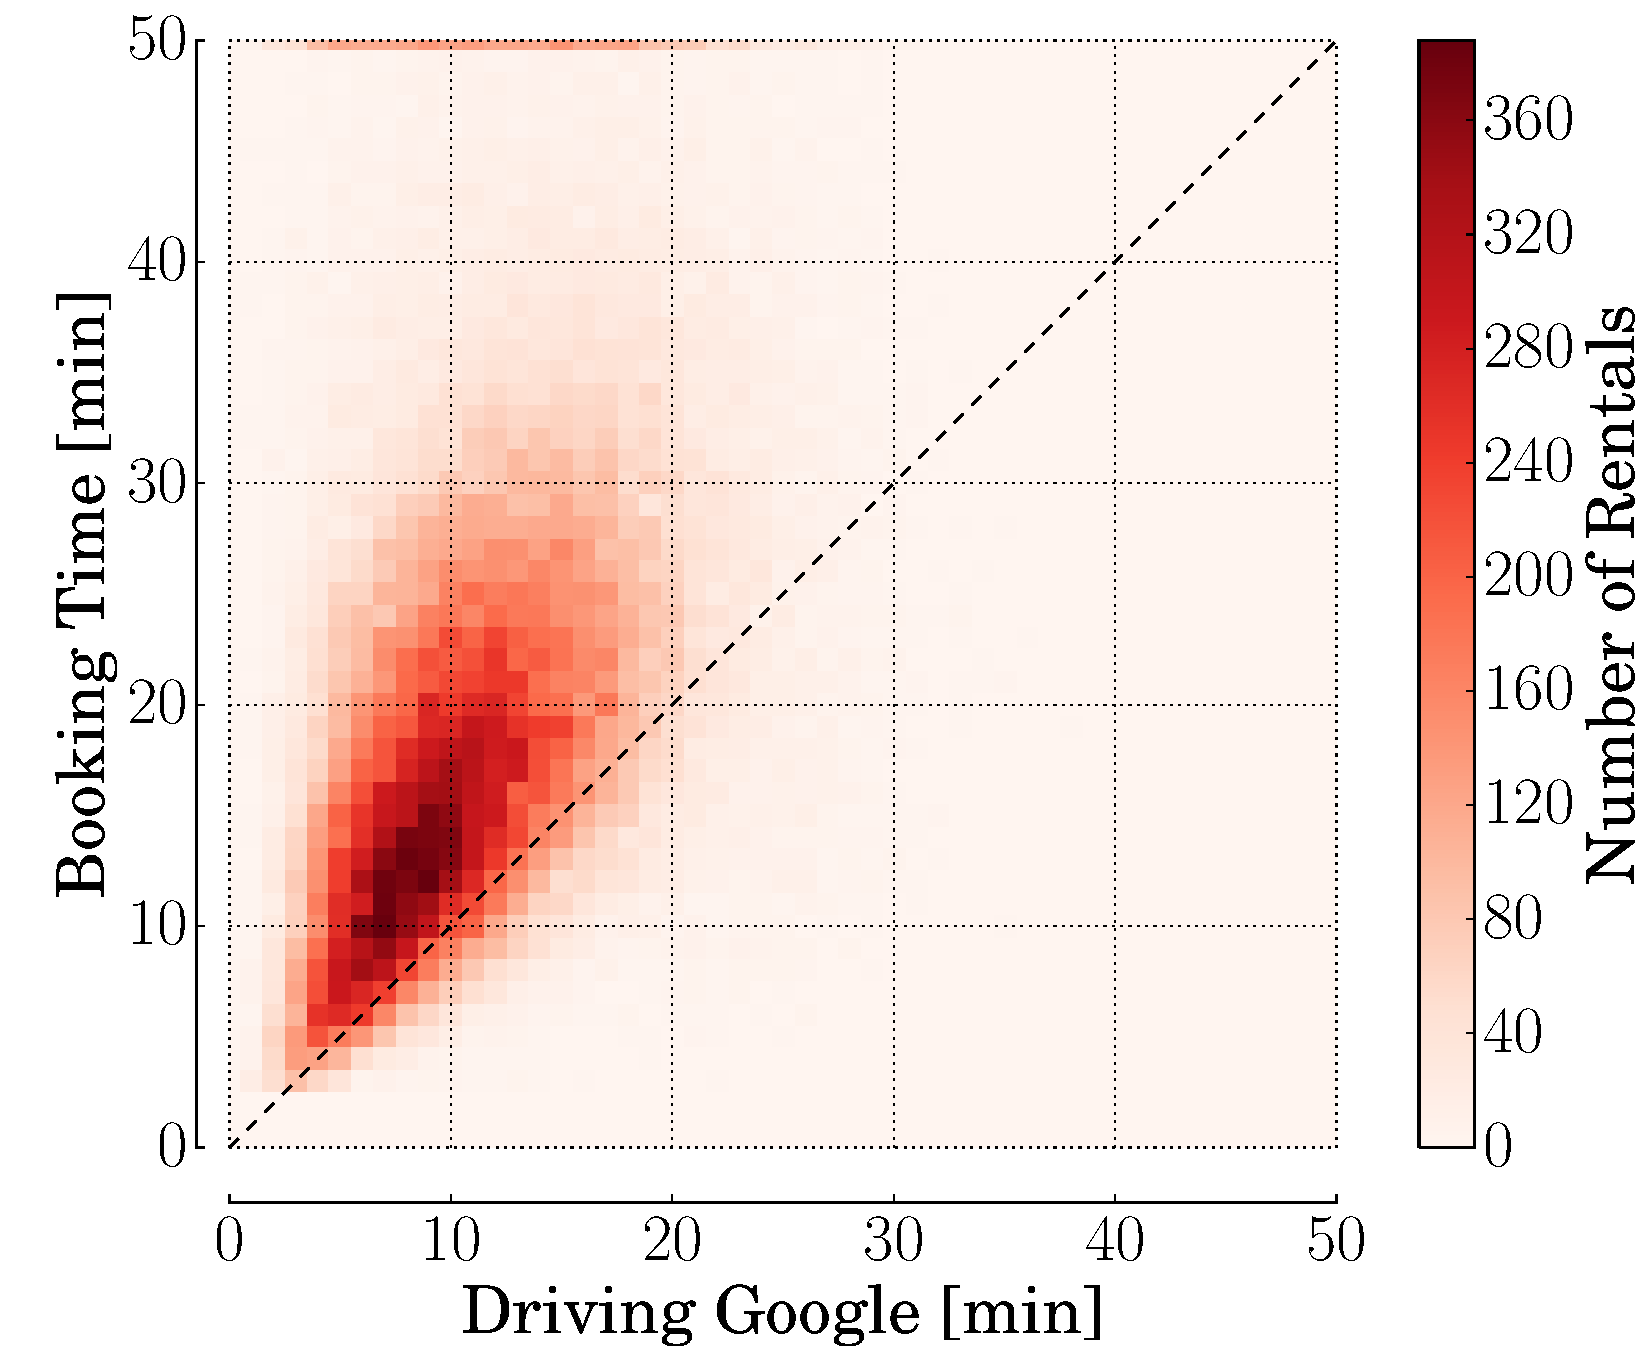
\includegraphics[width=0.5\columnwidth]{figures/car2go_faster_driving.pdf}}
%\subfloat[][ECDF of the difference between the expected driving time and the actual driving time]{\label{fig:cdf_faster_google}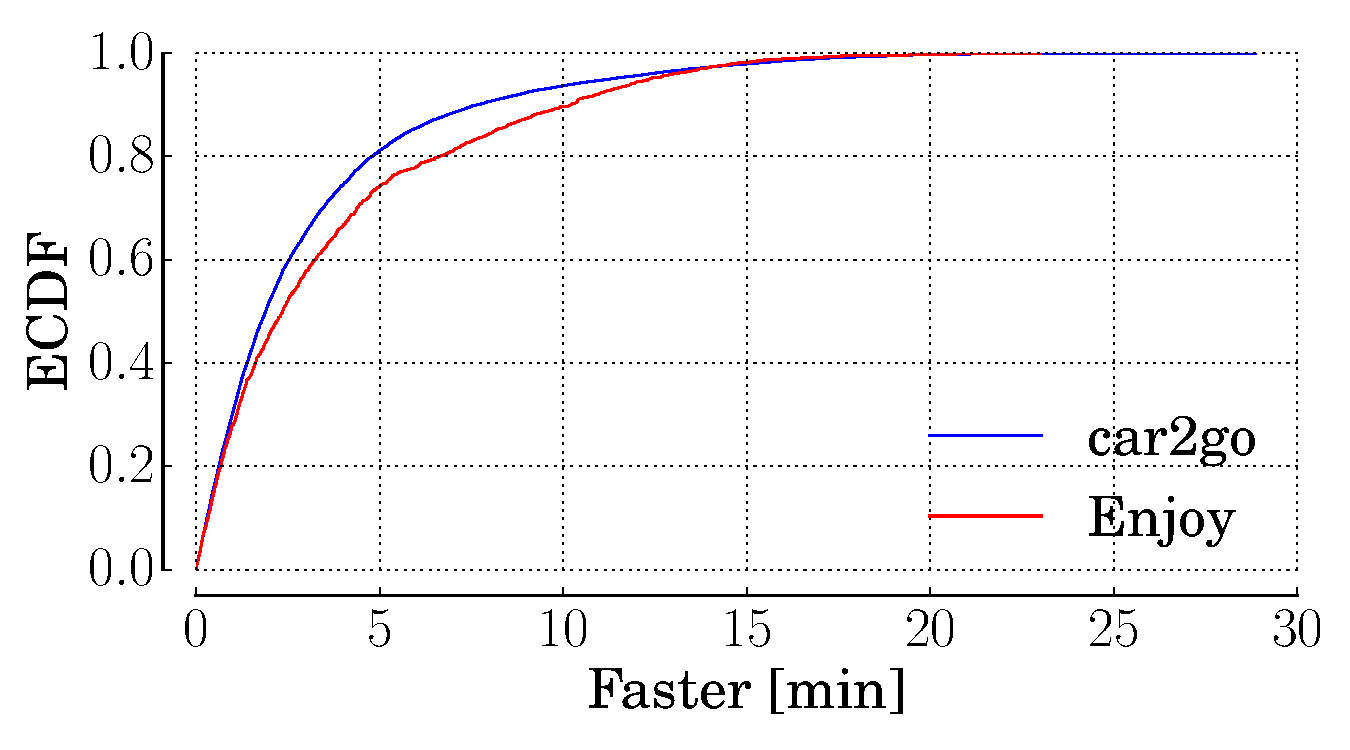
\includegraphics[width=0.5\columnwidth]{figures/faster_driving.pdf}}
%\caption{Users' driving habits}
%\end{figure}


At last, I leverage Google Directions APIs to extract public transport travel information for each vehicle's trip. I want to analyse another way of mobility in the urban area, and compare car sharing usage with respect to public transport. Results are shown in Figure~\ref{fig:3_5_public_transport}.
%The public transport duration includes both the time of travel and time of wait.
As one could expect, the majority of trips last less than public transport. The higher density is for bookings that last between 10 and 20 minutes. For longer trips, the discrepancy in terms of duration is higher, probably due to the longer path and the higher number of stops of the public transport. Conversely, I can interpret the points where the booking time is greater than  the public transport duration as trips where the customers spent a lot of time in reaching the car or finding a parking spot for the drop-off.

\begin{figure}[h!]
	\centering
	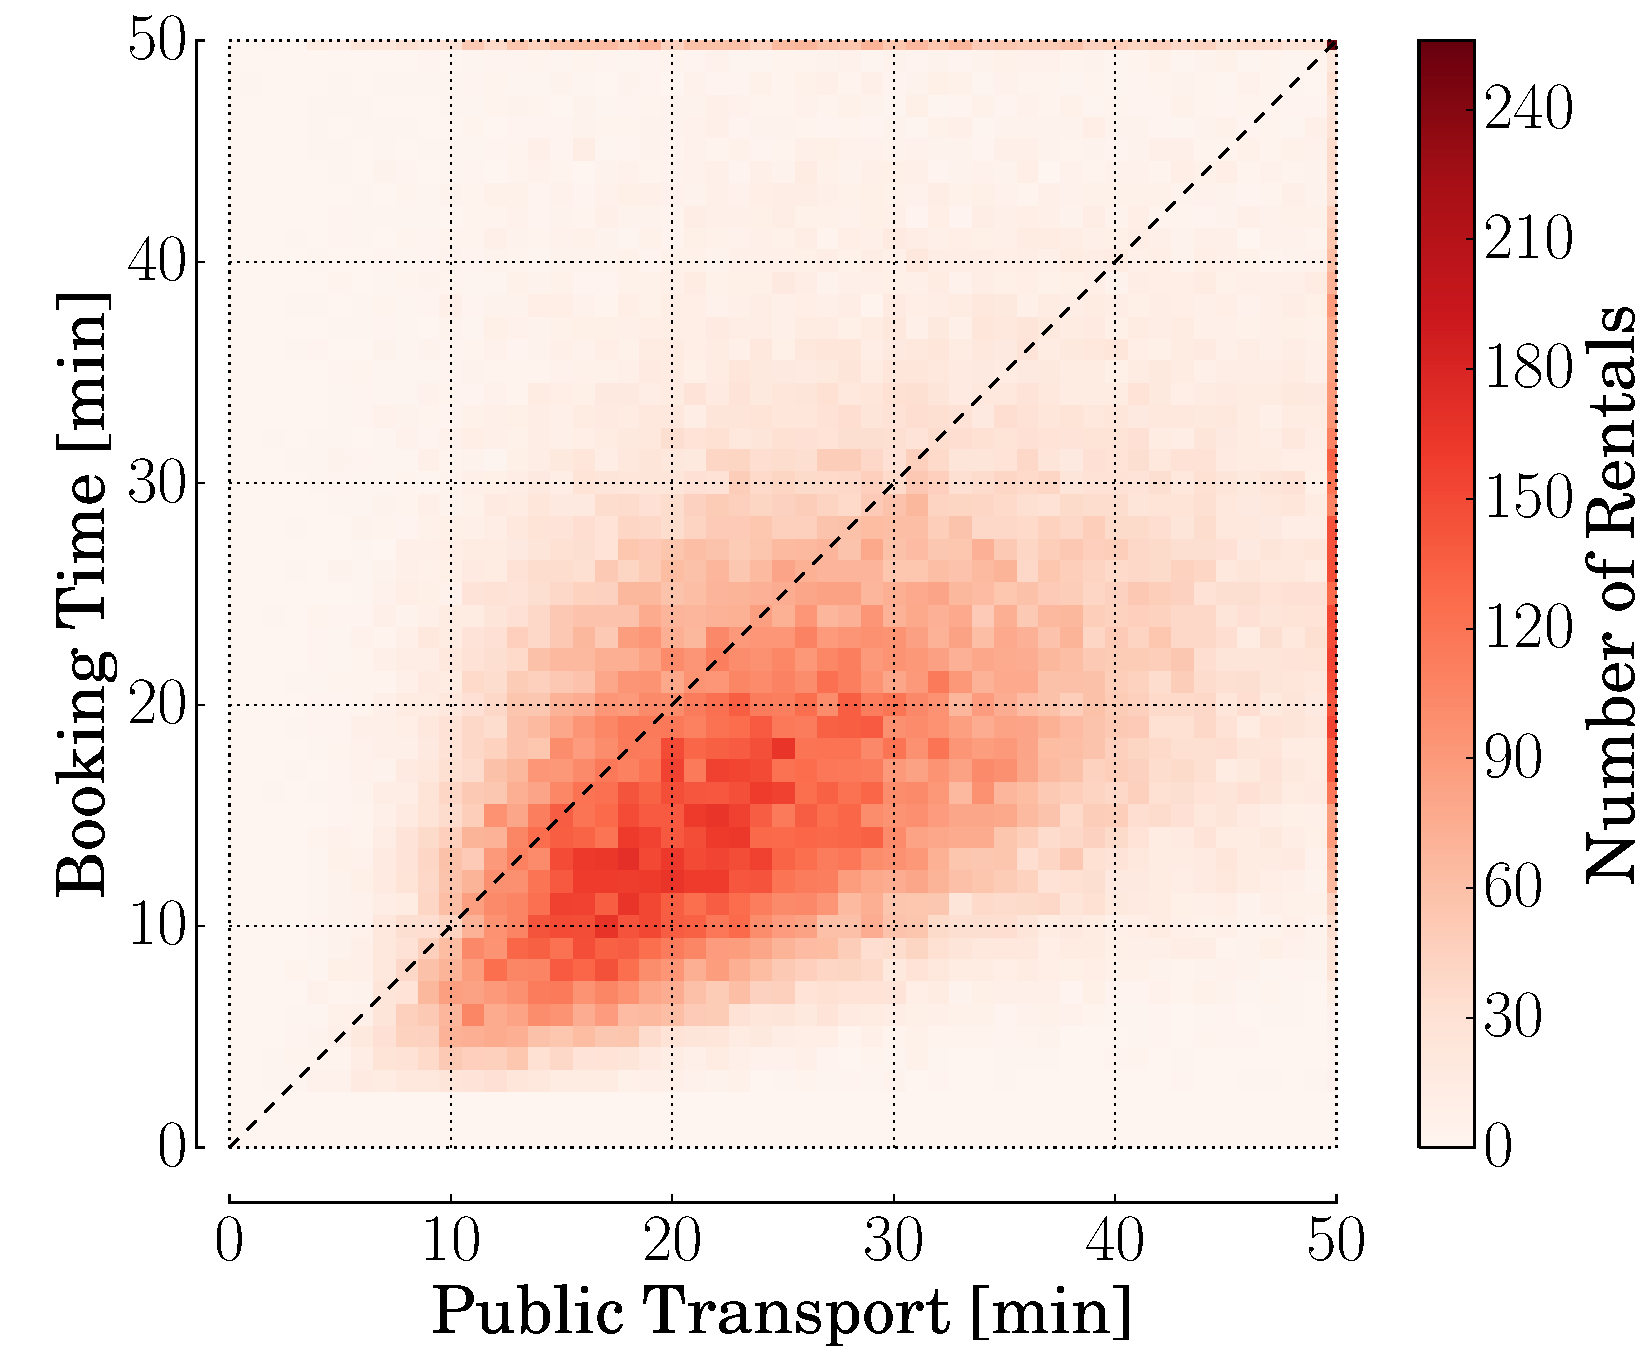
\includegraphics[width=0.85\columnwidth]{figures/car2go_faster_public.pdf}
	\caption{heatmap of the booking time  vs the estimated public transport time by Google\label{fig:3_5_public_transport}}
\end{figure}

To help to visualize the juxtaposition of car sharing and public transport, we extract from the data the probability of booking a car, conditioned to the public transport travel time. Figure~\ref{fig:pdf_transport}, reports on the X axis the public transport duration (as predicted by Google) in intervals of 5 minutes, and on the Y axis the probability of booking a car for each interval.
The distribution of probability is similar for both car2go and Enjoy. Higher values are reported for trips that can be covered by public transport between 15 and 35 minutes. Interestingly, car sharing mobility is not preferred for very short trips, while the distribution shows a significant tail for duration greater than 30 minutes. This behavior can be justified by the significant amount of time that can be saved with cars haring with respect to public transport.

\begin{figure}[h!]
	\centering
	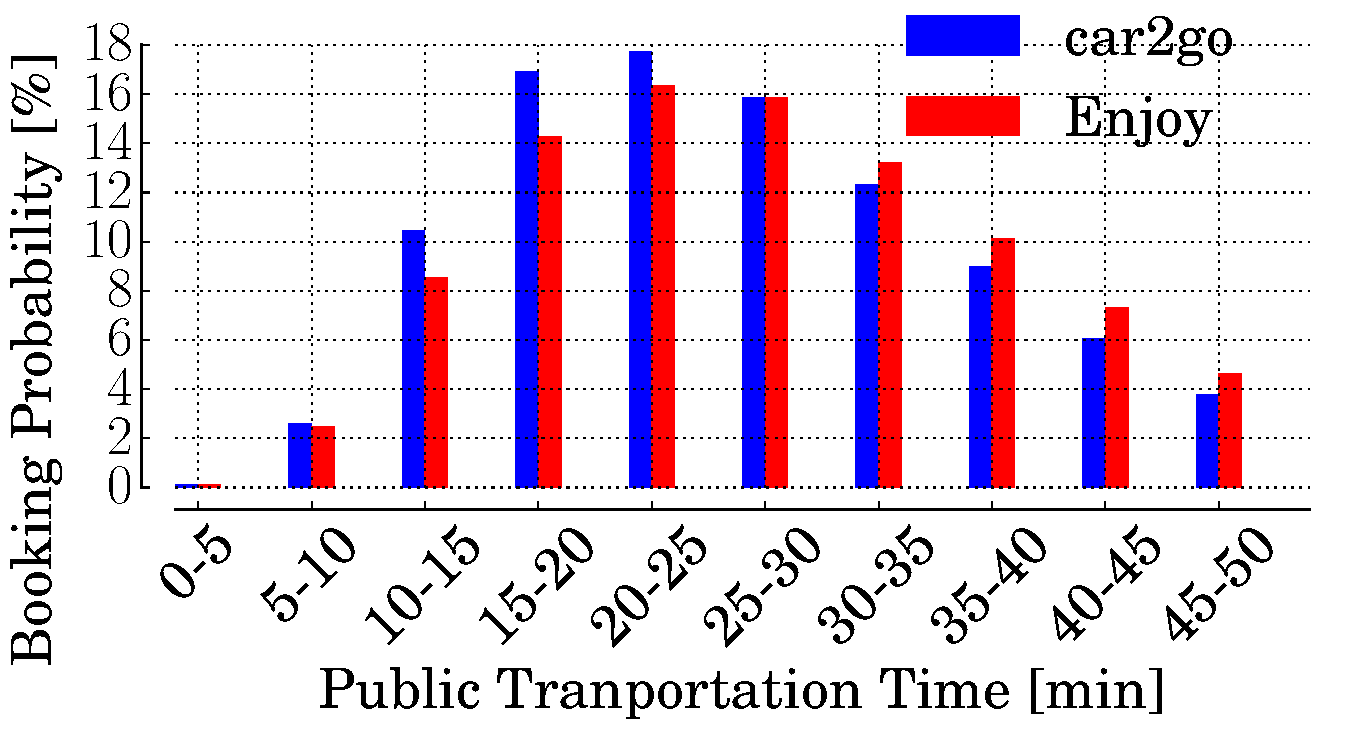
\includegraphics[width=0.85\columnwidth]{figures/public_tranport_probability.pdf}
	\caption{Public transportation vs car sharing\label{fig:3_5_public_tranport_probabilityt}}
\end{figure}
  
%  \begin{figure}[t!]
%  \centering     %%% not \center
%  \subfloat[][heatmap of the booking time  vs the estimated public tranport time by Google]{\label{fig:heatmap_transport}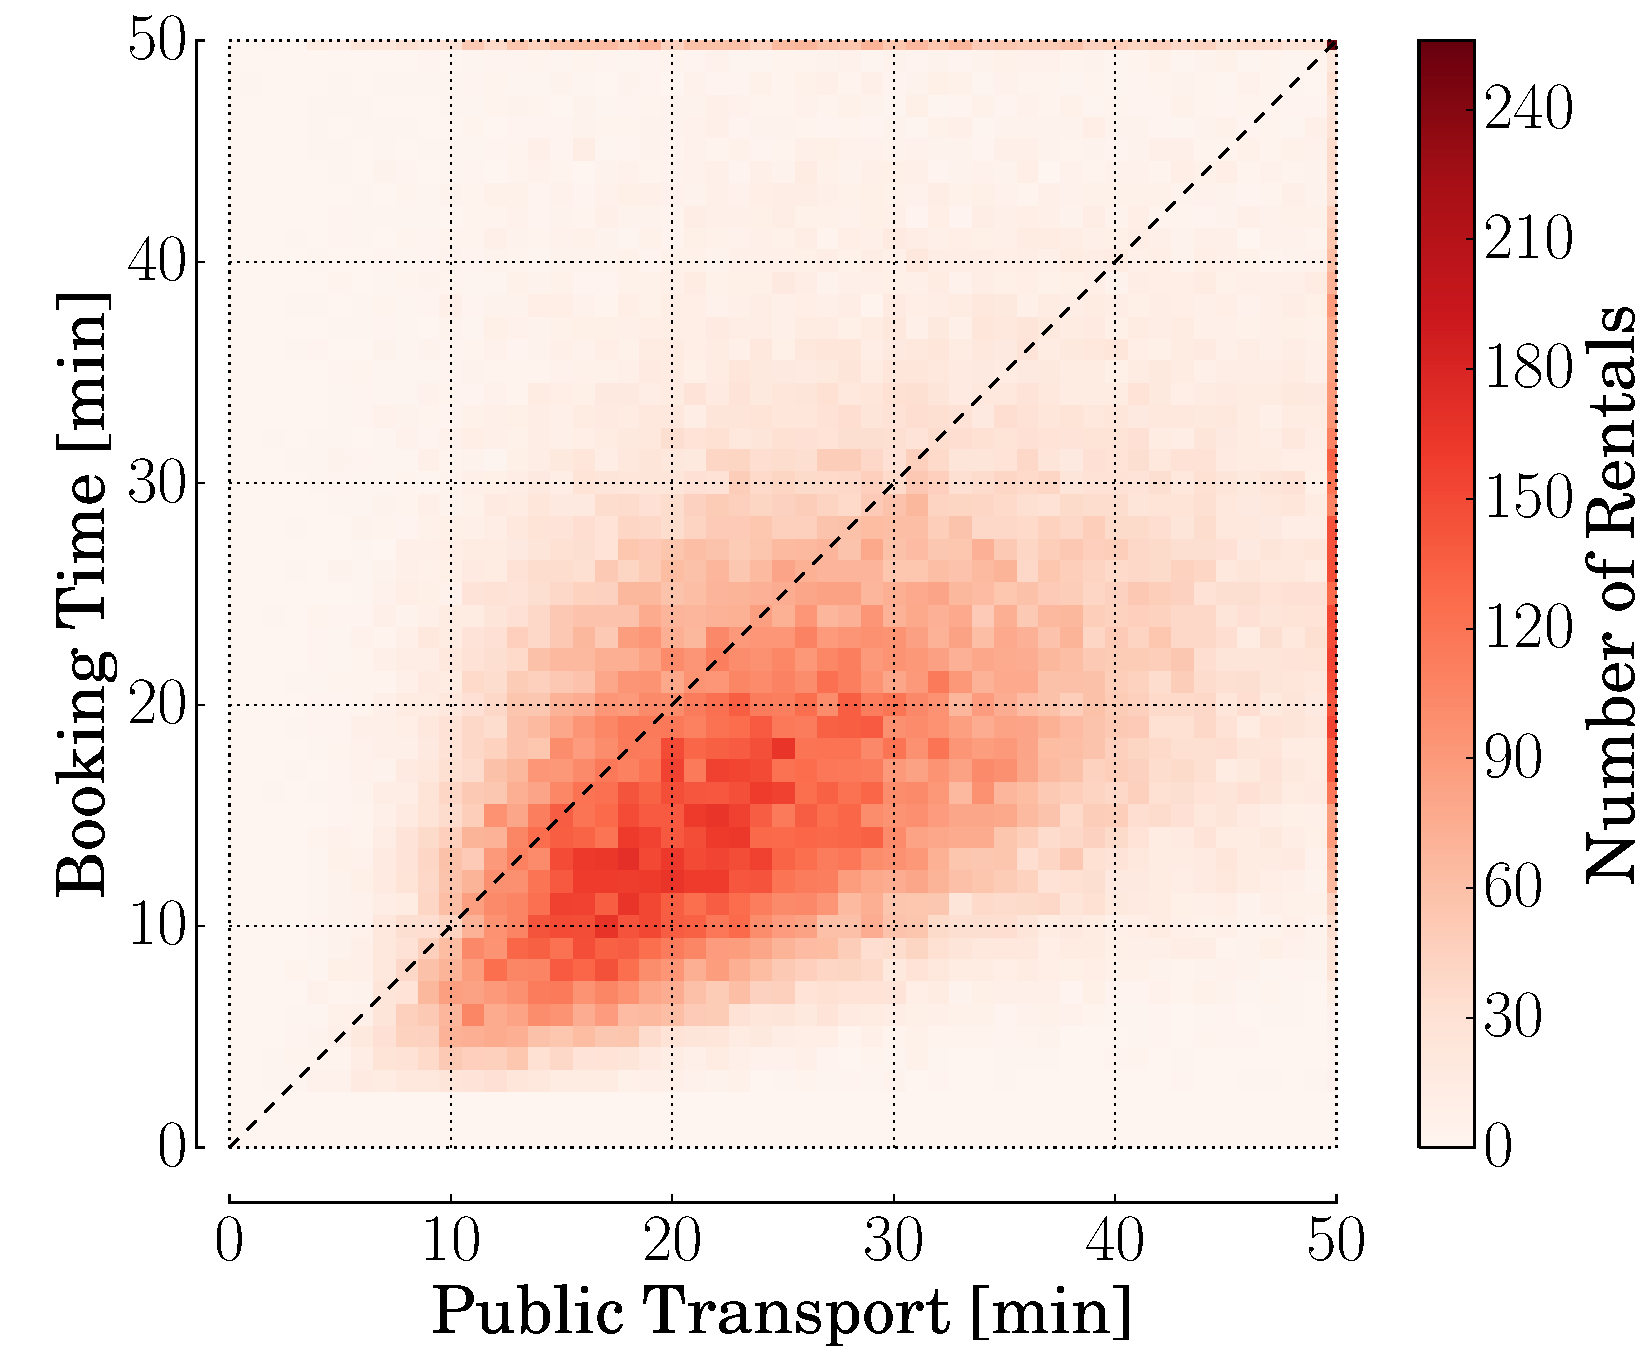
\includegraphics[width=0.5\columnwidth]{figures/car2go_faster_public.pdf}}
%  \subfloat[][Probability of using car sharing based on public transport time by Google]{\label{fig:pdf_transport}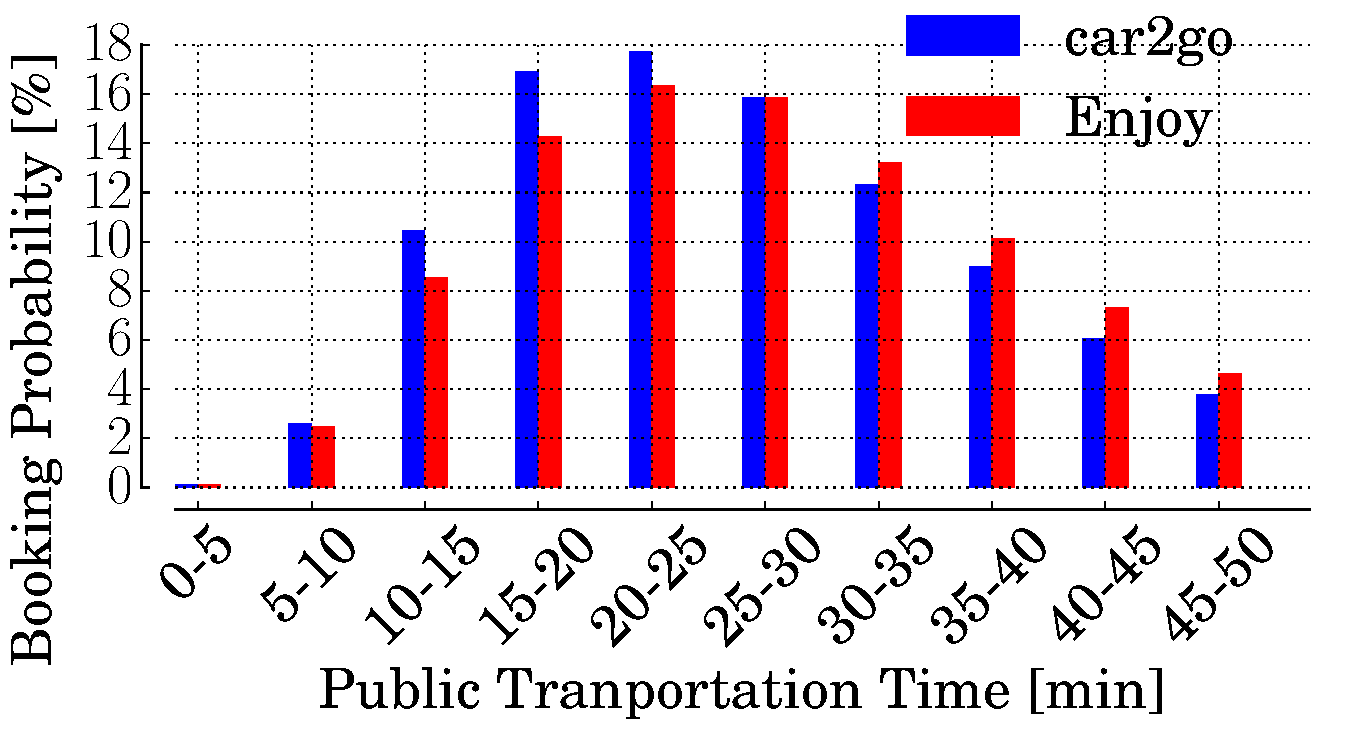
\includegraphics[width=0.5\columnwidth]{figures/public_tranport_probability.pdf}}
%  \caption{Public transportation vs car sharing \label{fig:public_transport}}
%  \end{figure}
%  
  
 
Finally, to globally understand how users tend to use the different services we report in Figure~\ref{fig:avg_comparison} the average time for: the Enjoy rentals (red curve), the car2go bookings (blue curve), the driving time (green curve), and public transport time (orange curve). To compute this value, for each hour we take all the rentals of interest, and then we compute the average value and report it. A first interesting aspect is that the average time of Enjoy is always greater then the car2go ones and for the pure driving time. Secondly, both show a similar trend with, a decreasing average duration during the night. As a consequence, it is unjustifiable ascribe this trend with traffic jam, instead, but more likely with an increase time in the reservation time and in the parking time. Finally, it is possible to appreciate how during the night the public transport takes more than 1 hour for trips which last less then 20 minutes by car. Instead, during the daytime the average public transport time get close to the car sharing time. 
%This demonstrates the goodness of the public transport system.



\begin{figure}[h!]
\centering
 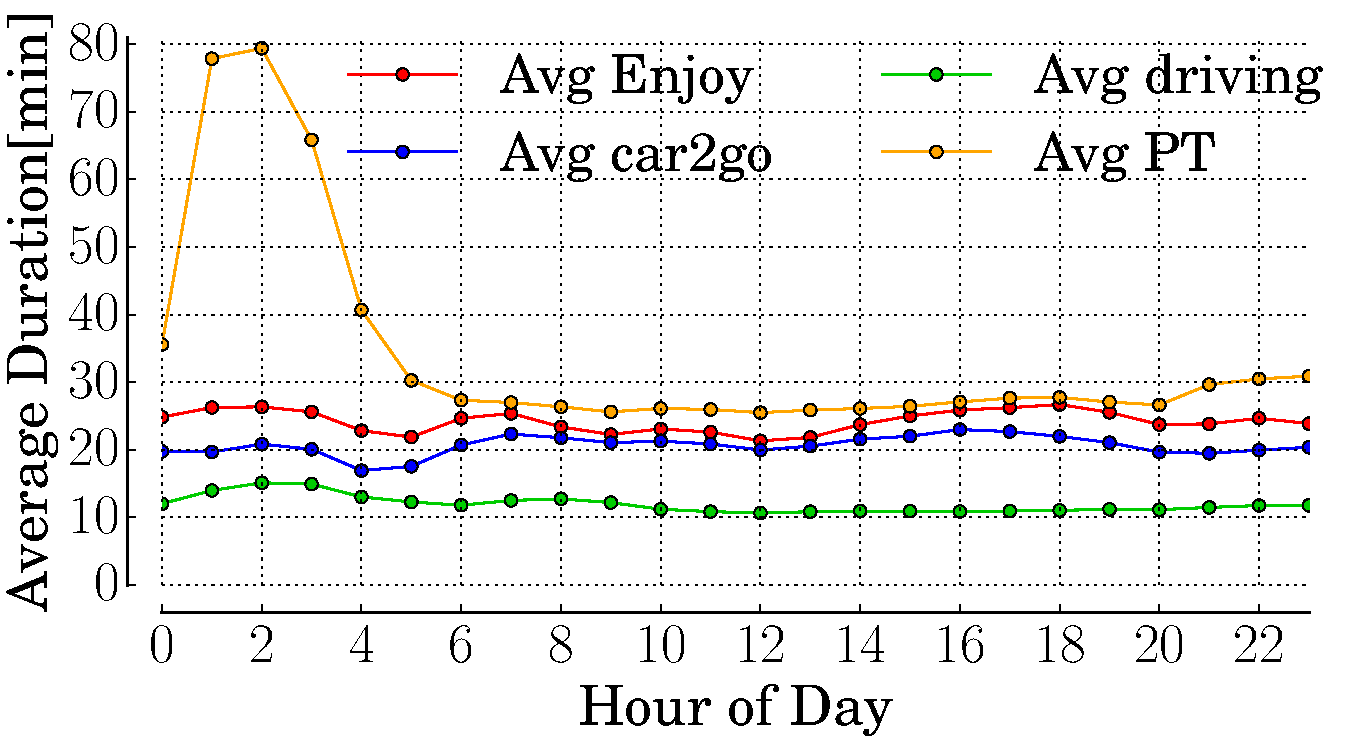
\includegraphics[width=0.85\columnwidth]{figures/average_duration.pdf}
 \caption{Average Time per transport solution per hour \label{fig:avg_comparison}}
\end{figure}



\section{Conclusions} 
\label{sec:3_6_conclusion}

In this article, we characterized three distinct car-sharing systems which operate in  Vancouver  (Canada)  and nearby regions. Our study, using data of more than one year of real trips, uncovers patterns of users’ habits.  We provided a characterization of the different car-sharing services, including spatial-temporal usage. Finally, we highlighted the main differences and the common characteristics of these services.

We showed that in Vancouver in 2017 the one-way and free-floating services were used similarly. They present shorter travels when compared to the two-way service. All three services present peaks of demand during the day. During working days, these peaks occur at around 8\,AM and 6\,PM, while in weekends, peaks are distributed in the afternoon. The two-way service we analyze presents a considerable number of booking cancellations and a higher vehicle idle time. This indicates a low utilization of the vehicles, likely due to their business model. Indeed, one-way and free-floating services allow users to pick-up a car and leave it anywhere in the city, dynamically satisfying the floating demand. 
We also highlight the strong relationship with the public transportation system, as well as with points of interests such as public universities and commercial centers.  Finally, we believe the characterization we provide may be used as a substrate for urban centers planning.

\section*{Acknowledgements}

The authors would like to thank CAPES, CNPq, FAPEMIG for their financial support in this research.

%% Numbered appendices remain in the main matter...
%\appendix
%\include{Appendix1/appendix1}
%\include{Appendix2/appendix2}

\backmatter% here begins the back matter
% ... otherwise a single appendix may stay here
%\include{References/biblio}

% Do not use this command if you did not prepare a nomenclature
% database by means of the suitable \nomenclature command and its
% arguments, as we did in chapter 2 of this example thesis.
\printnomencl

% In this example we use \nocite{*} in order to typeset the whole
% contents of the bibliographic database. Normally this is not
% necessary and it's better to let biber extract from the database
% only the cited works
%\nocite{*}


\printbibliography[heading=bibintoc]

% Do not use this command if you did not set the \makeindex switch
% in the preamble.

\printindex

\end{document}

